\documentclass[11pt]{article}

\usepackage[margin=1in]{geometry}
\usepackage{graphicx}
\usepackage{amsmath}
\usepackage{amssymb}
\usepackage{booktabs}
\usepackage{xcolor}
\usepackage[colorlinks=true,linkcolor=blue!55!black,urlcolor=blue!55!black,
            citecolor=blue!55!black]{hyperref}
\usepackage{caption}
\usepackage{float}
\usepackage{enumitem}

\captionsetup{font=small,labelfont=bf}
\setlist{itemsep=2pt,topsep=4pt}

\title{\textbf{Linking Reports to Information Needs with a Cross-Encoder}\\[4pt]
\large Supervised learning with pairwise attention over reports and need
justifications,\\ trained on author citations}

\author{Johnny Morgan\\ \small University of Maryland, Baltimore County}
\date{\today}

\begin{document}
\maketitle

\begin{abstract}
\noindent
We hold roughly 20,000 reports and more than 1,000 information needs. Each need
carries a written justification saying what would satisfy it. The link between
the two comes from authors: when an author writes that a report satisfies a
need, that citation is our label. We want a model that reads a new report and
predicts which needs it satisfies, and that surfaces report-need relationships
nobody has cited yet.

The obvious approach is to treat the need identifiers as class labels and train
a classifier on the report text alone. That approach throws away the
justifications, which is where most of the usable signal lives, and it cannot
score a need that did not exist at training time. We take a different approach.
We feed the report and a candidate justification into one transformer as a
single sequence, so that attention runs across both of them, and we train the
model to answer a yes-or-no question: does this report satisfy this need? The
base model is DistilBERT-MNLI, which already knows how to judge whether one
passage supports another.

One property of the data shapes everything downstream. A citation is a reliable
positive, but the absence of a citation is not a negative. It means nobody has
written the link down, which covers both irrelevance and undiscovered relevance.
This is positive-unlabeled learning, and it has a consequence worth stating
early: the uncited pairs the model scores highly are the discoveries we are
after, yet a naive evaluation counts them as errors.

This paper explains supervised learning from the beginning, then attention and
transformers, then what pairwise attention means and why it is the right tool
here. It gives a concrete schema for the training data, covers pair construction
and negative sampling under positive-unlabeled conditions, the loss function,
evaluation for the multi-label case, a discovery loop that converts model output
into new labels, and how to serve the model against a repository of this size.
It closes with the failure modes we expect and how we would detect them.
\end{abstract}

\tableofcontents
\newpage

%======================================================================
\section{The problem}

An information need is a standing statement of what someone is trying to find
out. In a reference library it might be a patron's underlying question behind a
search query. In an analytic organisation it is a documented requirement that
stays open across many documents. Either way it has two parts: a short label,
and a longer justification written in prose that says what would count as
satisfying it.

We hold three things:

\begin{enumerate}
  \item \textbf{A report corpus.} Reports $r_1 \ldots r_N$, with $N \approx
        20{,}000$.
  \item \textbf{A need repository.} Needs $n_1 \ldots n_M$, each with a written
        justification $j_1 \ldots j_M$, with $M > 1{,}000$.
  \item \textbf{A citation record.} Rows saying that an author cited report
        $r_i$ as satisfying need $n_j$. This is where our labels come from.
\end{enumerate}

The candidate space is therefore $N \times M \approx 20$ million report-need
pairs, of which the cited ones are a very thin slice. A report can satisfy
several needs at once, and satisfies none of the overwhelming majority.

We want two things from the model. First, given a new report, return the needs
it satisfies. Second, and this is the harder one, surface report-need pairs that
are real but that nobody has cited. Section~\ref{sec:discovery} deals with the
second.

The question this paper answers is how to build that function so that it
actually reads the justifications, rather than memorising which identifier tends
to co-occur with which vocabulary.

Why does that distinction matter? Because a model trained on identifiers alone
learns nothing that transfers to a need it has never seen. Add a new need to the
repository tomorrow and the model has no output for it, no training examples for
it, and no way to score it without a full retraining run. Over 1,000 needs, with
new ones opening over time, that is a treadmill. A model that reads
justifications can score a brand new need the moment someone writes its
justification down. That property is worth designing for.

%======================================================================
\section{Supervised learning}

Supervised learning fits a function to labelled examples. We start with pairs
$(x_i, y_i)$ where $x_i$ is an input and $y_i$ is the correct answer. We pick a
family of functions $f_\theta$ controlled by parameters $\theta$, and we search
for the $\theta$ that makes $f_\theta(x_i)$ close to $y_i$ across the training
set.

``Close'' needs a definition, and that definition is the \textbf{loss function}
$L(\hat{y}, y)$. It takes the model's prediction and the true answer and returns
a single number that is small when they agree and large when they do not. The
whole training procedure is a search for parameters that make this number small.

The search itself is \textbf{gradient descent}. We compute
$\nabla_\theta L$, the direction in parameter space that increases the loss
fastest, and step the opposite way:

\begin{equation}
\theta \leftarrow \theta - \eta \, \nabla_\theta L
\end{equation}

\noindent where $\eta$ is the learning rate, a small number controlling step
size. We do this over mini-batches. Computing the gradient across millions of
examples for every step is wasteful, and the noise from small batches turns out
to help. Figure~\ref{fig:loop} shows the
loop.

\begin{figure}[H]
\centering
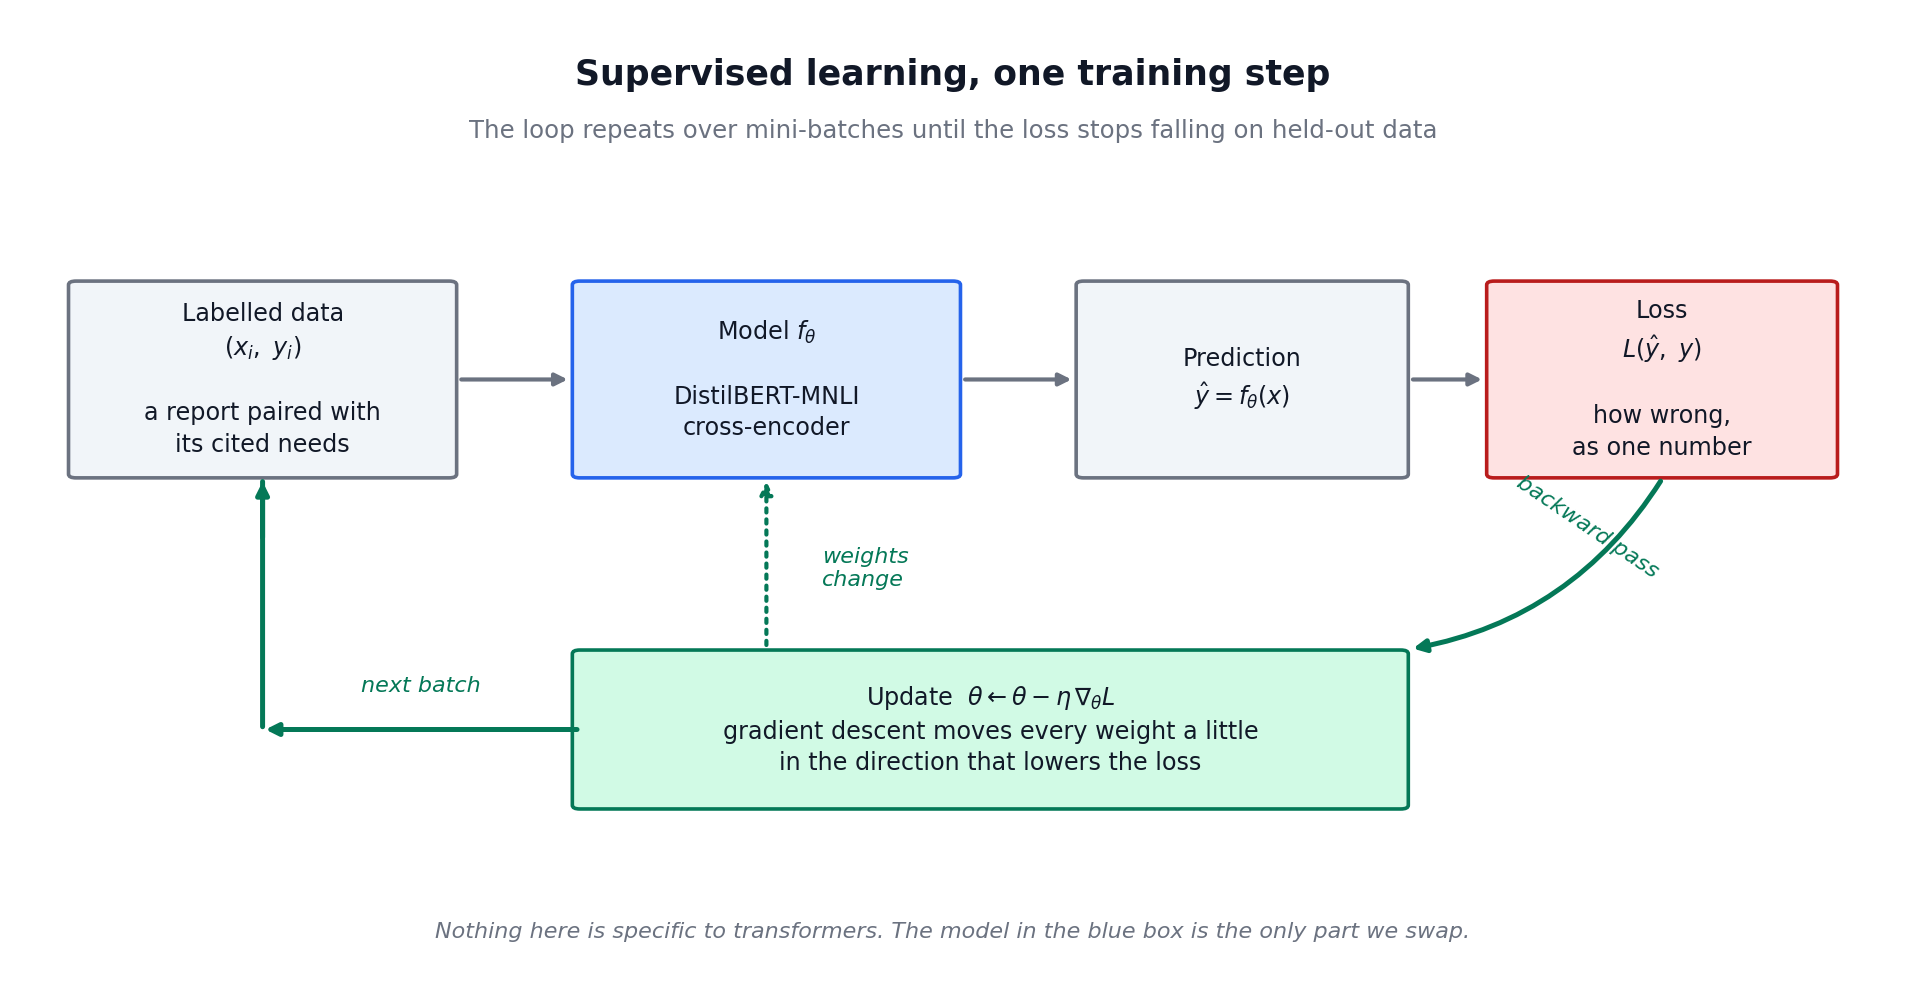
\includegraphics[width=\textwidth]{figures/fig01_supervised_loop.png}
\caption{One step of supervised training. The model is the only component that
changes when we switch architectures. Everything else in this diagram is the
same whether the model is logistic regression or a transformer.}
\label{fig:loop}
\end{figure}

\subsection{Generalisation, and why we hold data back}

Fitting the training data is not the goal. The goal is performing well on texts
we have never seen. These two come apart, and the gap between them is called
\textbf{overfitting}: the model memorises quirks of the training set that do not
hold in general.

We guard against this by splitting the data three ways.

\begin{itemize}
  \item \textbf{Training set.} The model sees these and learns from them.
  \item \textbf{Validation set.} The model never trains on these. We use them to
        choose hyperparameters and decide when to stop training.
  \item \textbf{Test set.} Touched once, at the end, to report a number.
\end{itemize}

One warning specific to our setup. The split must be by \emph{text}, not by
pair. If the same text appears in training as a positive pair with need A and in
validation as a negative pair with need B, the model has seen that text during
training and the validation score is inflated. Split the texts first, then build
pairs within each split.

%======================================================================
\section{Where the label lives}

Here is the design decision that shapes everything downstream. The label is not
a property of the text. It is a property of the \textbf{pair}.

Instead of asking ``which of $M$ classes does this text belong to?'' we ask, for
each candidate need, ``does this text satisfy this need, yes or no?'' A text with
three gold needs produces three positive pairs and, in principle, $M-3$ negative
ones.

This reframing buys us three things:

\begin{enumerate}
  \item The justification text enters the model. It is half the input.
  \item Adding a need requires writing a justification, not retraining.
  \item The output is naturally multi-label. Each pair gets its own independent
        decision, and no softmax forces the needs to compete for probability
        mass.
\end{enumerate}

It costs us one thing, and the cost is real: inference now scales with $M$.
Section~\ref{sec:serving} deals with that.

%======================================================================
\section{Where the labels come from}
\label{sec:labels}

Our labels are citations. An author read a report, decided it satisfied a need,
and wrote that down. This is a better signal than most annotation projects
produce, because the judgement was made by someone doing real work with real
stakes, not by an annotator working through a queue.

It is also incomplete in a specific way, and the whole method has to account for
it.

\begin{quote}
A citation is a reliable \textbf{positive}. The absence of a citation is
\textbf{not a negative}. It is an absence of information.
\end{quote}

An uncited report-need pair can be any of three things. The report may be
irrelevant to the need, which is true of the vast majority. The report may be
relevant but the author cited a different report instead. Or the report may be
relevant and simply never connected to that need by anyone. Nothing in the data
distinguishes these cases.

\begin{figure}[H]
\centering
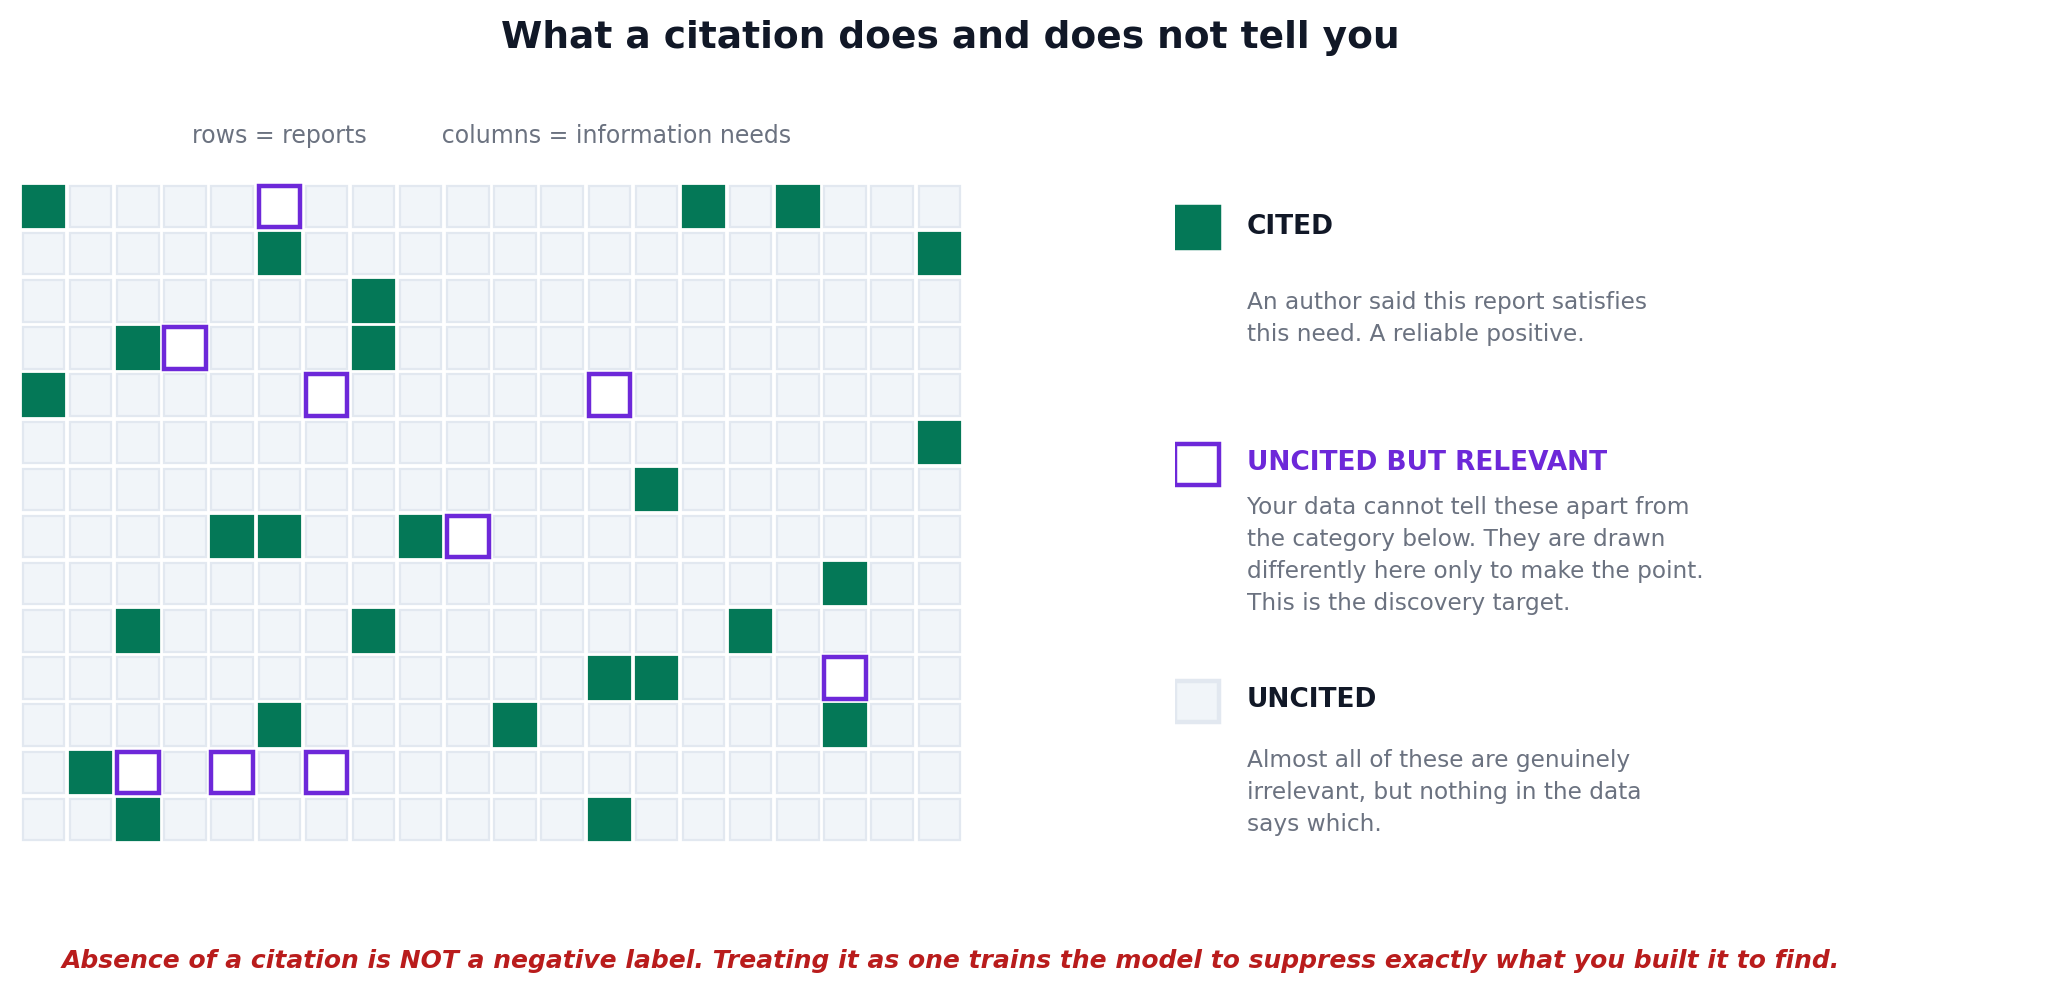
\includegraphics[width=\textwidth]{figures/fig11_citation_label_structure.png}
\caption{The label structure. Green cells are observed. Everything else is
unknown, and the unknown region contains both irrelevance and the relationships
we are trying to find.}
\label{fig:pu}
\end{figure}

This setting has a name: \textbf{positive-unlabeled learning}, meaning we have
confirmed positives and unlabeled everything-else, with no confirmed negatives
at all. Three consequences follow, and each shows up later in the paper.

\textbf{Sampled negatives are assumptions, not facts.} When we draw a negative
in Section~\ref{sec:trainset}, we are asserting that an uncited pair is
irrelevant. At 0.15\% citation density that assumption is right nearly always,
which is why the approach works. But it is wrong sometimes, and it is wrong most
often precisely on the pairs that look most relevant, which are the ones we draw
as hard negatives. Hard negative mining and false negative injection are the
same operation here. Section~\ref{sec:trainset} says what to do about it.

\textbf{Measured precision is a floor, not an estimate.} If the model flags an
uncited pair and that pair is genuinely relevant, the evaluation scores it as a
false positive. True precision is therefore at least the measured precision and
probably higher. Any comparison between two models is still valid, since both
are penalised the same way, but the absolute number understates the system.

\textbf{The errors are the product.} A high-scoring uncited pair is the output
you asked for. Section~\ref{sec:discovery} turns that from a metric problem into
a workflow.

%======================================================================
\section{Structuring the training data}
\label{sec:schema}

Three tables you curate and one the trainer derives. Keeping the derived table
derived matters: if anyone hand-edits pairs, the sampling policy stops being
reproducible and no two training runs are comparable.

\begin{figure}[H]
\centering
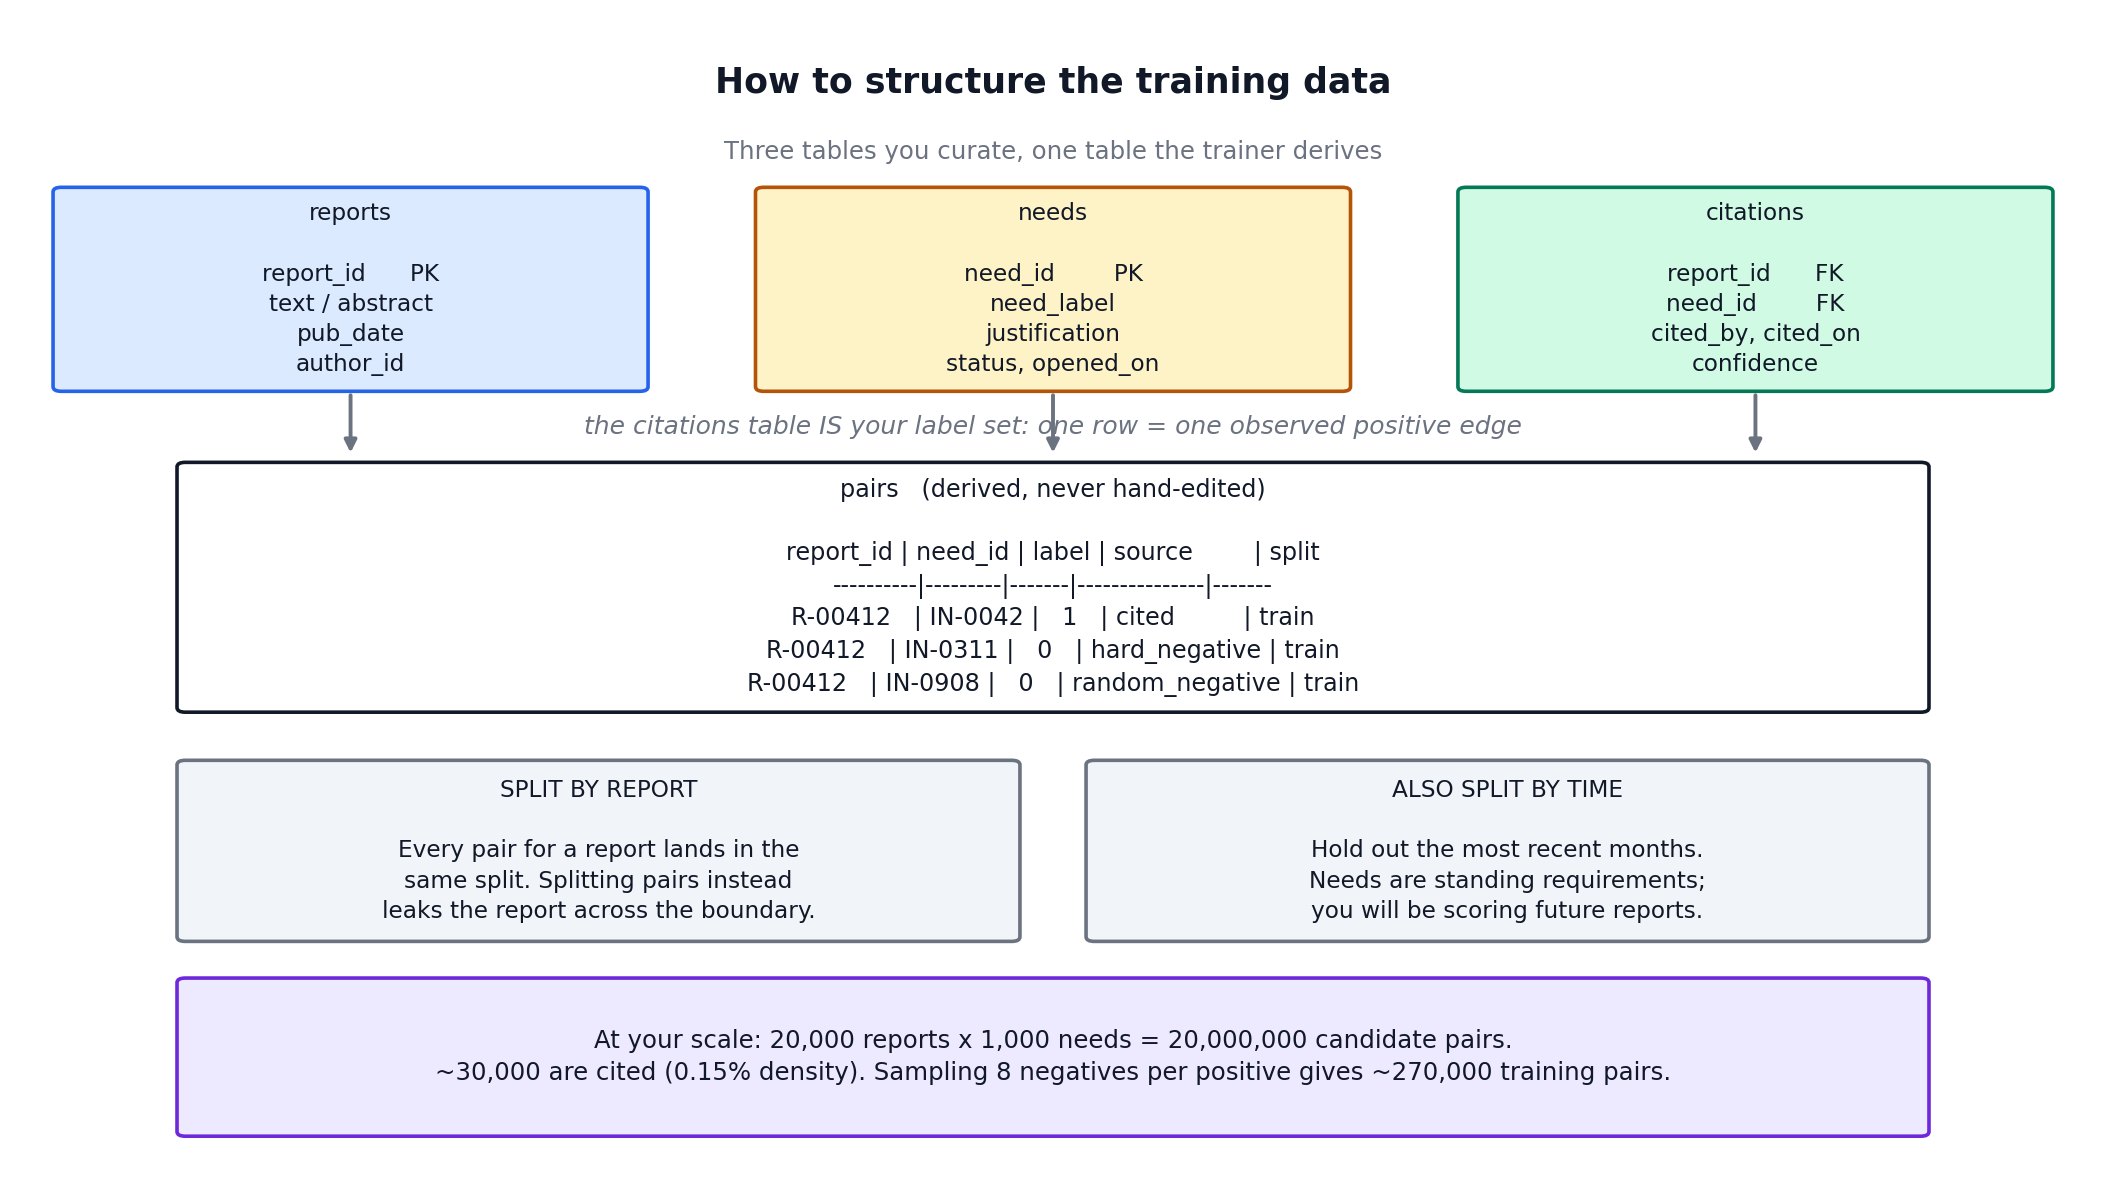
\includegraphics[width=\textwidth]{figures/fig12_data_structure.png}
\caption{The schema. The citations table is the label set; every row is one
observed positive edge.}
\label{fig:schema}
\end{figure}

Four fields are worth arguing for specifically.

\textbf{\texttt{citations.cited\_on}} lets you split by time. Needs are standing
requirements and reports arrive continuously, so the deployed model will score
documents written after everything it trained on. Hold out the most recent
months as a second test set and compare it against the random split. The gap
between them is your best estimate of how fast the model will decay in service.

\textbf{\texttt{citations.cited\_by}} lets you check whether the model has
learned an author rather than a need. If precision is much higher on citations
from one prolific author, the model may have learned that author's writing
habits. Group by author and compare.

\textbf{\texttt{needs.opened\_on}} lets you run the decisive test of the whole
design. Hold out every need opened after some date, train on the rest, and score
the held-out needs. Those needs contributed nothing to training, so performance
on them measures the thing the architecture was chosen for: whether a
justification alone is enough to classify against a need the model has never
seen. If that number is poor, the cross-encoder is not buying what it costs.

\textbf{\texttt{citations.confidence}}, if your record distinguishes a passing
mention from a central citation, gives you a way to weight positives. Start
without it. Add it only if error analysis shows weak citations are hurting.

\subsection{What the numbers work out to}

At $N = 20{,}000$ and $M = 1{,}000$ the candidate space is 20 million pairs. If
the citation record holds roughly 30,000 edges, density is about 0.15\%, so
sampling eight negatives per positive yields on the order of 270,000 training
pairs. At batch size 32 that is roughly 8,400 steps per epoch and about 25,000
steps for three epochs, which is a few hours on one P100 and well under an hour
on a modern card. This is a small training job. The expensive part of this
project is adjudication, not compute.

%======================================================================
\section{Building the training set}
\label{sec:trainset}

\begin{figure}[H]
\centering
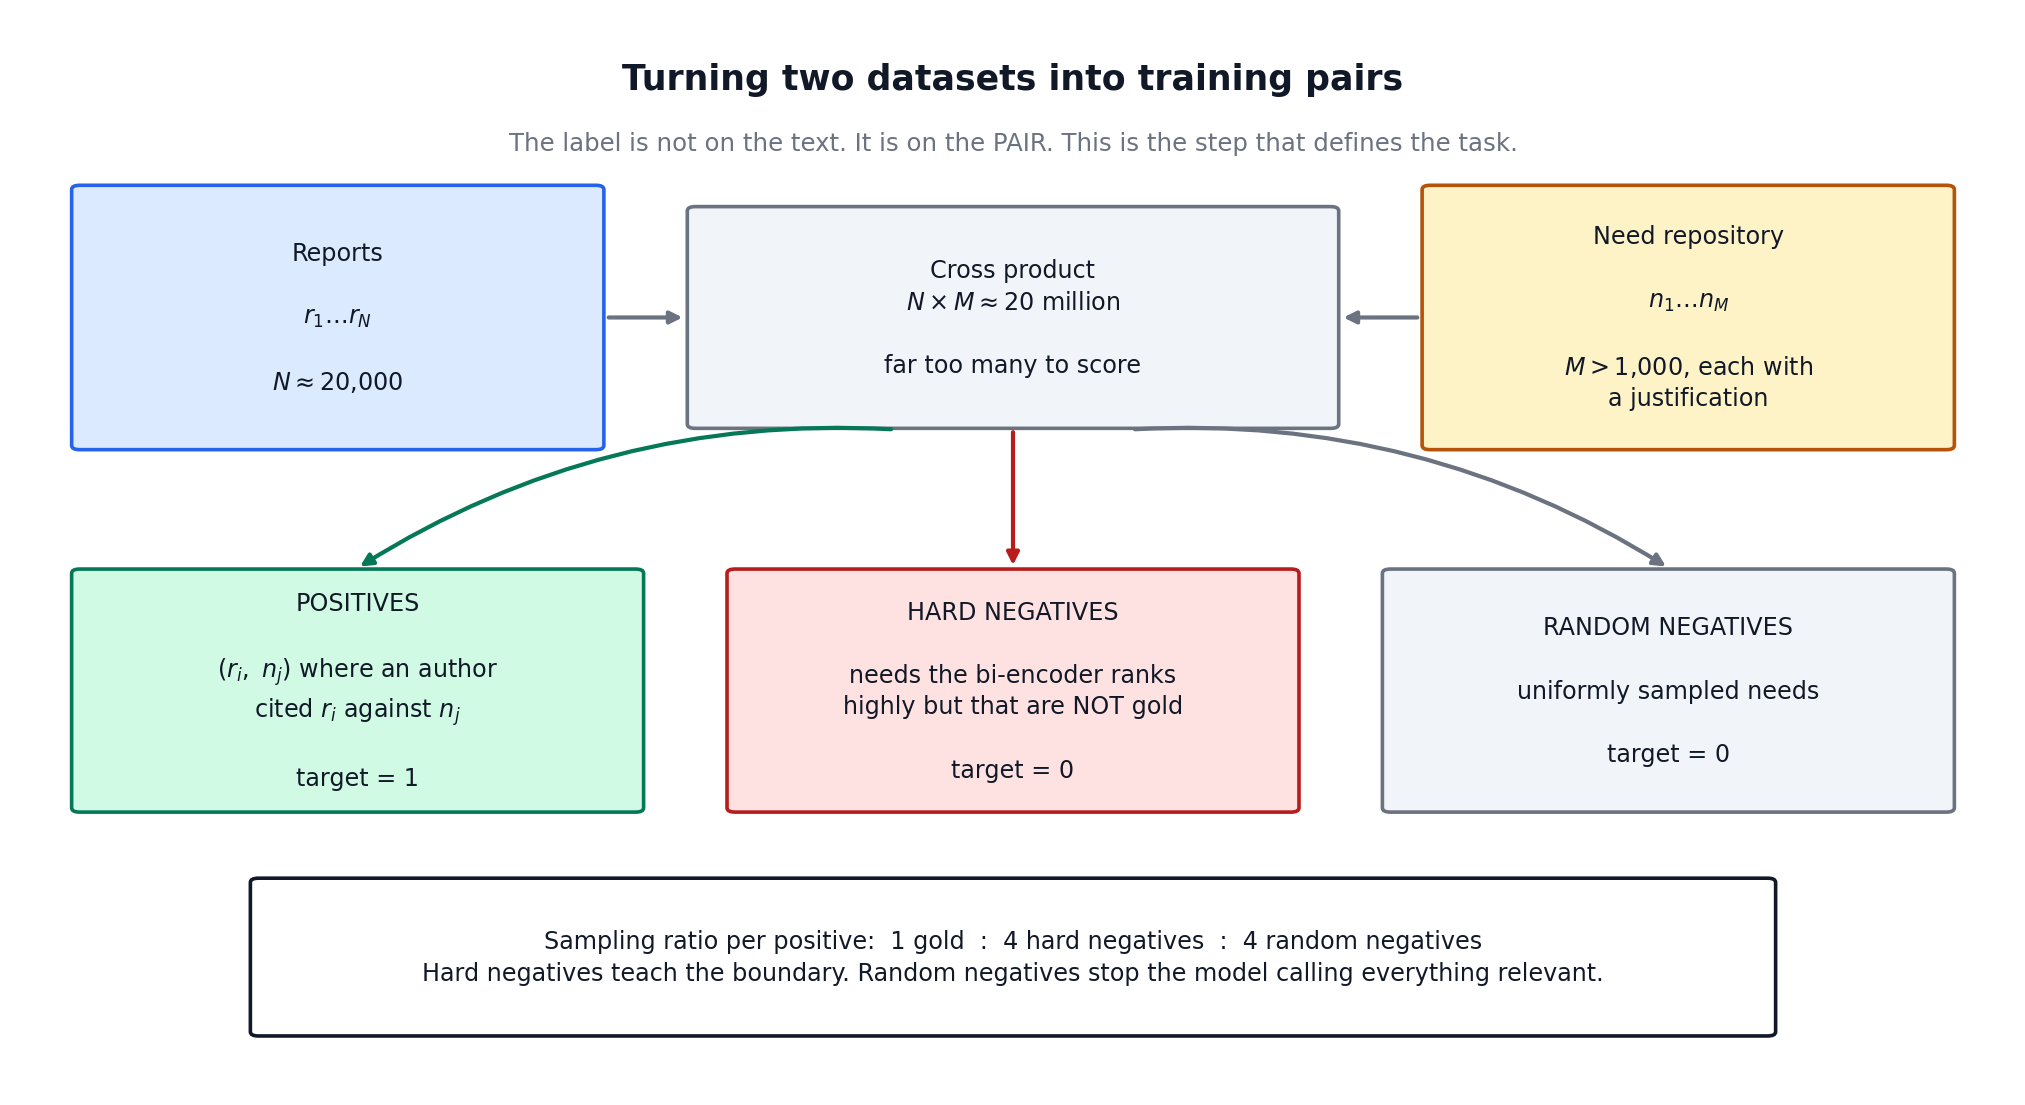
\includegraphics[width=\textwidth]{figures/fig06_pair_construction.png}
\caption{Building the training set. The cross product is far too large to
enumerate, so the sampling policy in the bottom box is part of the method and
not an implementation detail.}
\label{fig:pairs}
\end{figure}

\subsection{Negative sampling}

With $M > 1{,}000$ and a citation density near 0.15\%, the natural class balance
is roughly one positive to 660 unlabeled pairs. Train on that directly and the
model learns to answer ``no'' to everything, which scores 99.85\% accuracy and
is useless.

We sample instead. For every positive pair we draw:

\begin{itemize}
  \item \textbf{Four hard negatives.} Needs that a cheap retrieval model ranks
        highly for this text but that are not in the gold set. These sit near the
        decision boundary and are what actually teaches the model to
        discriminate.
  \item \textbf{Four random negatives.} Needs drawn uniformly. These stop the
        model from concluding that anything vaguely on-topic is relevant.
\end{itemize}

Hard negatives alone produce a model that is sharp near the boundary and
overconfident far from it. Random negatives alone produce a model that solves an
easy problem. The mixture matters more than the exact ratio, and 4:4 is a
starting point to tune, not a result.

One caution on hard negatives. If the retrieval model used to mine them is the
same model being trained, the two co-adapt and the negatives stop being
informative. Mine hard negatives with a separate frozen retriever, or re-mine
them once between epochs, and record which you did.

\subsection{The tension hard negatives create here}

Section~\ref{sec:labels} said sampled negatives are assumptions. Hard negative
mining makes that assumption at its weakest point on purpose. A hard negative is
by construction a pair the retriever thinks looks relevant, which is exactly the
description of an uncited-but-relevant pair. So the sharper the mining, the more
often we teach the model that a real relationship is not one.

Three ways to manage it, in increasing order of effort.

\textbf{Skip the very top of the ranking.} Draw hard negatives from ranks 10 to
50 instead of 1 to 10. The top few candidates for a report are where genuine
uncited relevance concentrates. This costs almost nothing and is where to start.

\textbf{Soften the targets.} Train hard negatives against a target of 0.1 rather
than 0.0, which is label smoothing applied to one class. The model still learns
to rank them below positives without being told they are impossible.

\textbf{Feed adjudication back.} Every pair a human confirms as irrelevant in
Section~\ref{sec:discovery} becomes a negative you actually know. Over rounds,
the sampled negatives get replaced by confirmed ones where it matters most.

Whichever you choose, record it. The negative sampling policy is the single
most consequential decision in this design and it is invisible in the trained
weights.

\begin{figure}[H]
\centering
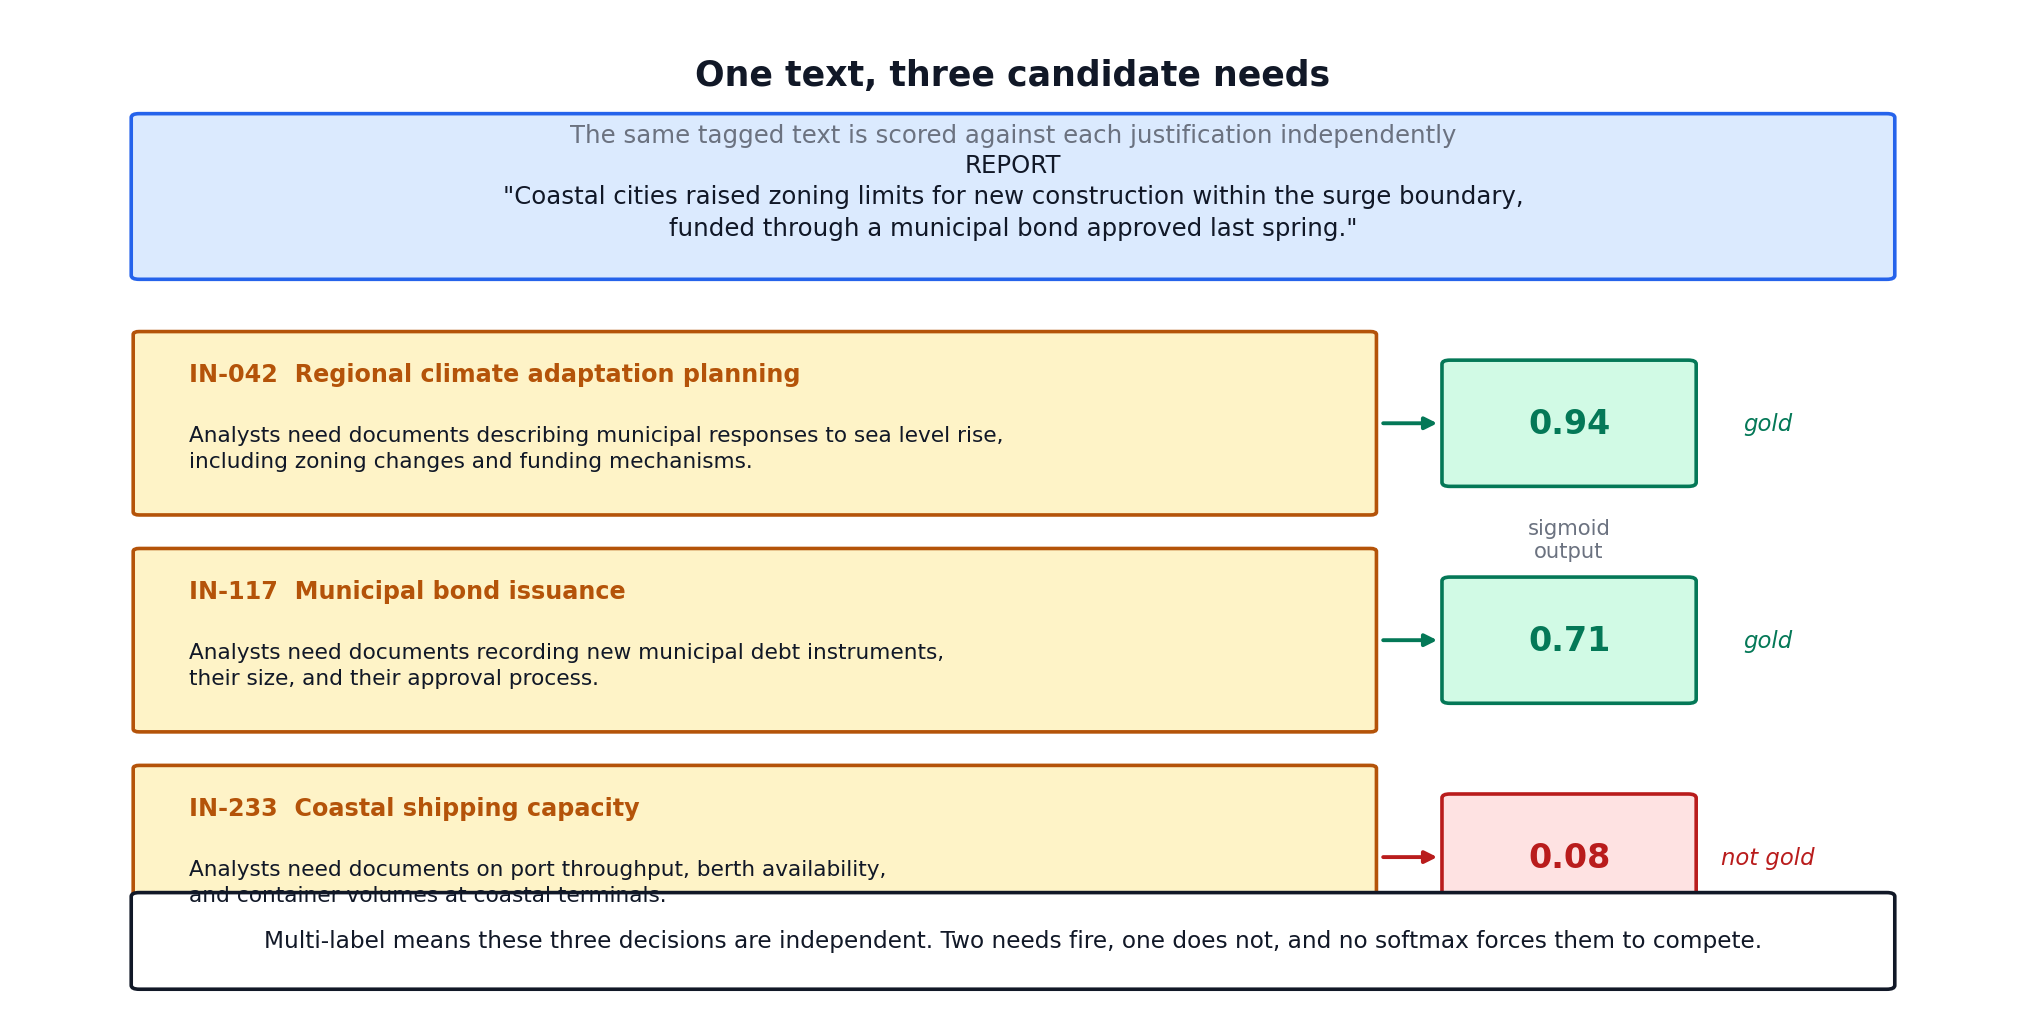
\includegraphics[width=\textwidth]{figures/fig10_worked_example.png}
\caption{One text scored against three candidate needs. The third is a plausible
distractor: it shares the vocabulary of coasts and cities but concerns port
throughput, which the text does not discuss. Distractors of this kind are
exactly what hard negative mining is for.}
\label{fig:example}
\end{figure}

%======================================================================
\section{Transformers and attention}

A transformer turns a sequence of tokens into a sequence of vectors, where each
output vector is informed by every other token in the sequence. The mechanism
that does the informing is attention.

\subsection{Tokens and embeddings}

Text first becomes tokens. DistilBERT uses WordPiece, which splits rare words
into sub-word units, so ``zoning'' might stay whole while an unusual proper noun
becomes three pieces. Each token maps to a learned vector of 768 numbers. A
position embedding is added so the model can tell word order, since attention
itself is order-blind.

\subsection{Query, key, value}

Each token vector is projected three ways using learned matrices, producing a
\textbf{query} $q$, a \textbf{key} $k$, and a \textbf{value} $v$. The intuition
is a soft lookup table. The query says what this token is looking for. The key
says what this token offers. The value is what this token contributes if
selected.

To compute the output for a token, we take the dot product of its query with
every key in the sequence, giving a score per token. We scale the scores, run
them through a softmax so they become weights summing to one, and take the
weighted average of the values. Stacked over all tokens at once:

\begin{equation}
\mathrm{Attention}(Q, K, V) = \mathrm{softmax}\!\left(\frac{Q K^{\top}}{\sqrt{d_k}}\right) V
\end{equation}

The division by $\sqrt{d_k}$ keeps the dot products from growing with dimension
and pushing the softmax into a region where its gradients vanish.

\begin{figure}[H]
\centering
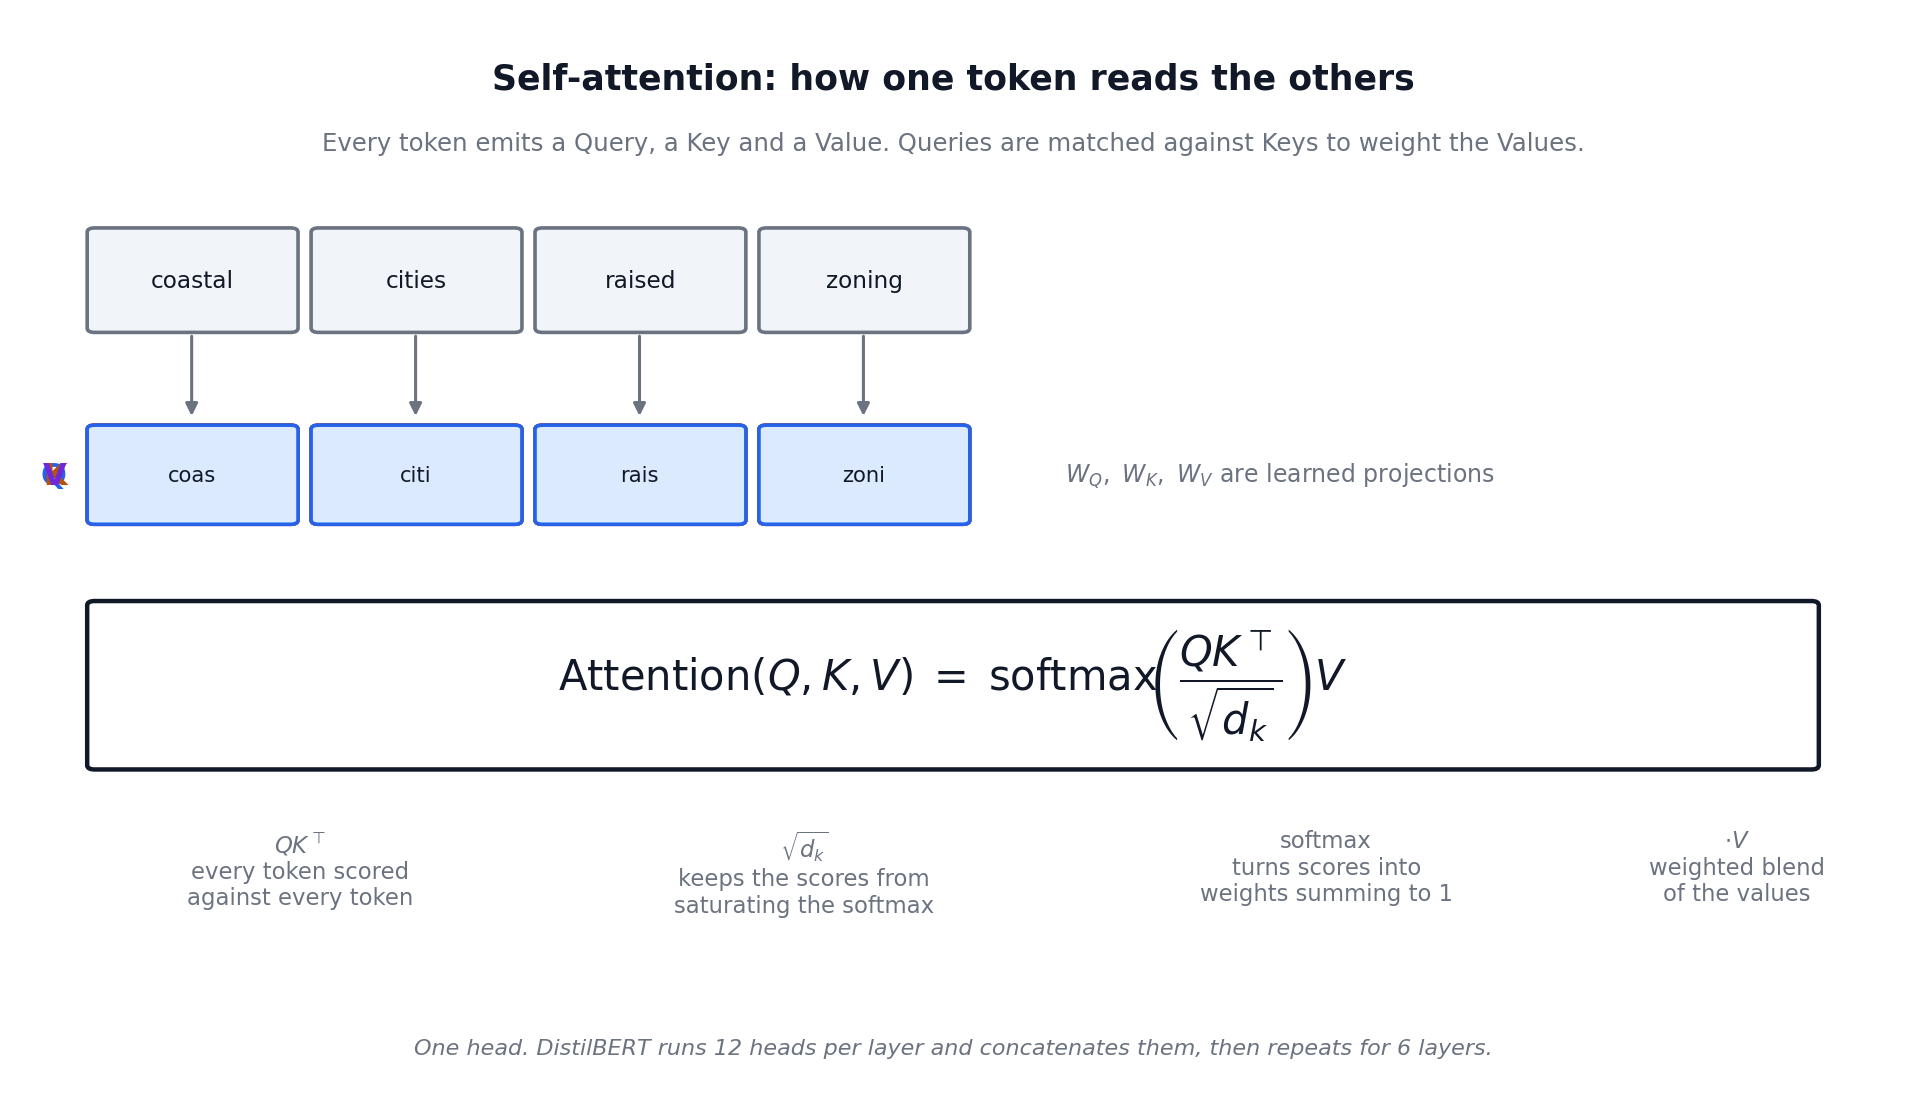
\includegraphics[width=\textwidth]{figures/fig02_attention_mechanism.png}
\caption{Self-attention for one head. DistilBERT runs twelve heads in parallel
per layer, concatenates their outputs, and repeats through six layers. Different
heads learn different relations: some track syntax, some track coreference, some
appear to do very little.}
\label{fig:attn}
\end{figure}

The matrix $QK^{\top}$ is the object to hold onto. It is $n \times n$ for a
sequence of $n$ tokens, and entry $(i,j)$ says how much token $i$ attends to
token $j$. The next section is entirely about the shape of that matrix.

%======================================================================
\section{Pairwise attention}

Now the central idea. We want the model to compare a text against a
justification. Where should that comparison happen?

\subsection{Two places it could happen}

One option is to encode each side separately into a vector and compare the
vectors, usually with a cosine similarity. This is a \textbf{bi-encoder}. The
comparison happens \emph{after} encoding, at a single dot product.

The other option is to concatenate both sides into one sequence and encode them
together. This is a \textbf{cross-encoder}. The comparison happens \emph{during}
encoding, at every layer, between every pair of tokens.

We build the input like this:

\begin{center}
\texttt{[CLS] coastal cities raised zoning limits [SEP] municipal response to sea level rise [SEP]}
\end{center}

\noindent \texttt{[CLS]} is a special token whose final vector is used as the
summary of the whole pair. \texttt{[SEP]} marks the boundary. A segment
embedding is added to every token recording which side it came from, so the
model knows which half is the text and which is the justification.

Because attention is computed over the whole sequence, the $n \times n$
attention matrix now has four regions, and two of them span the boundary.
Figure~\ref{fig:cross} shows this.

\begin{figure}[H]
\centering
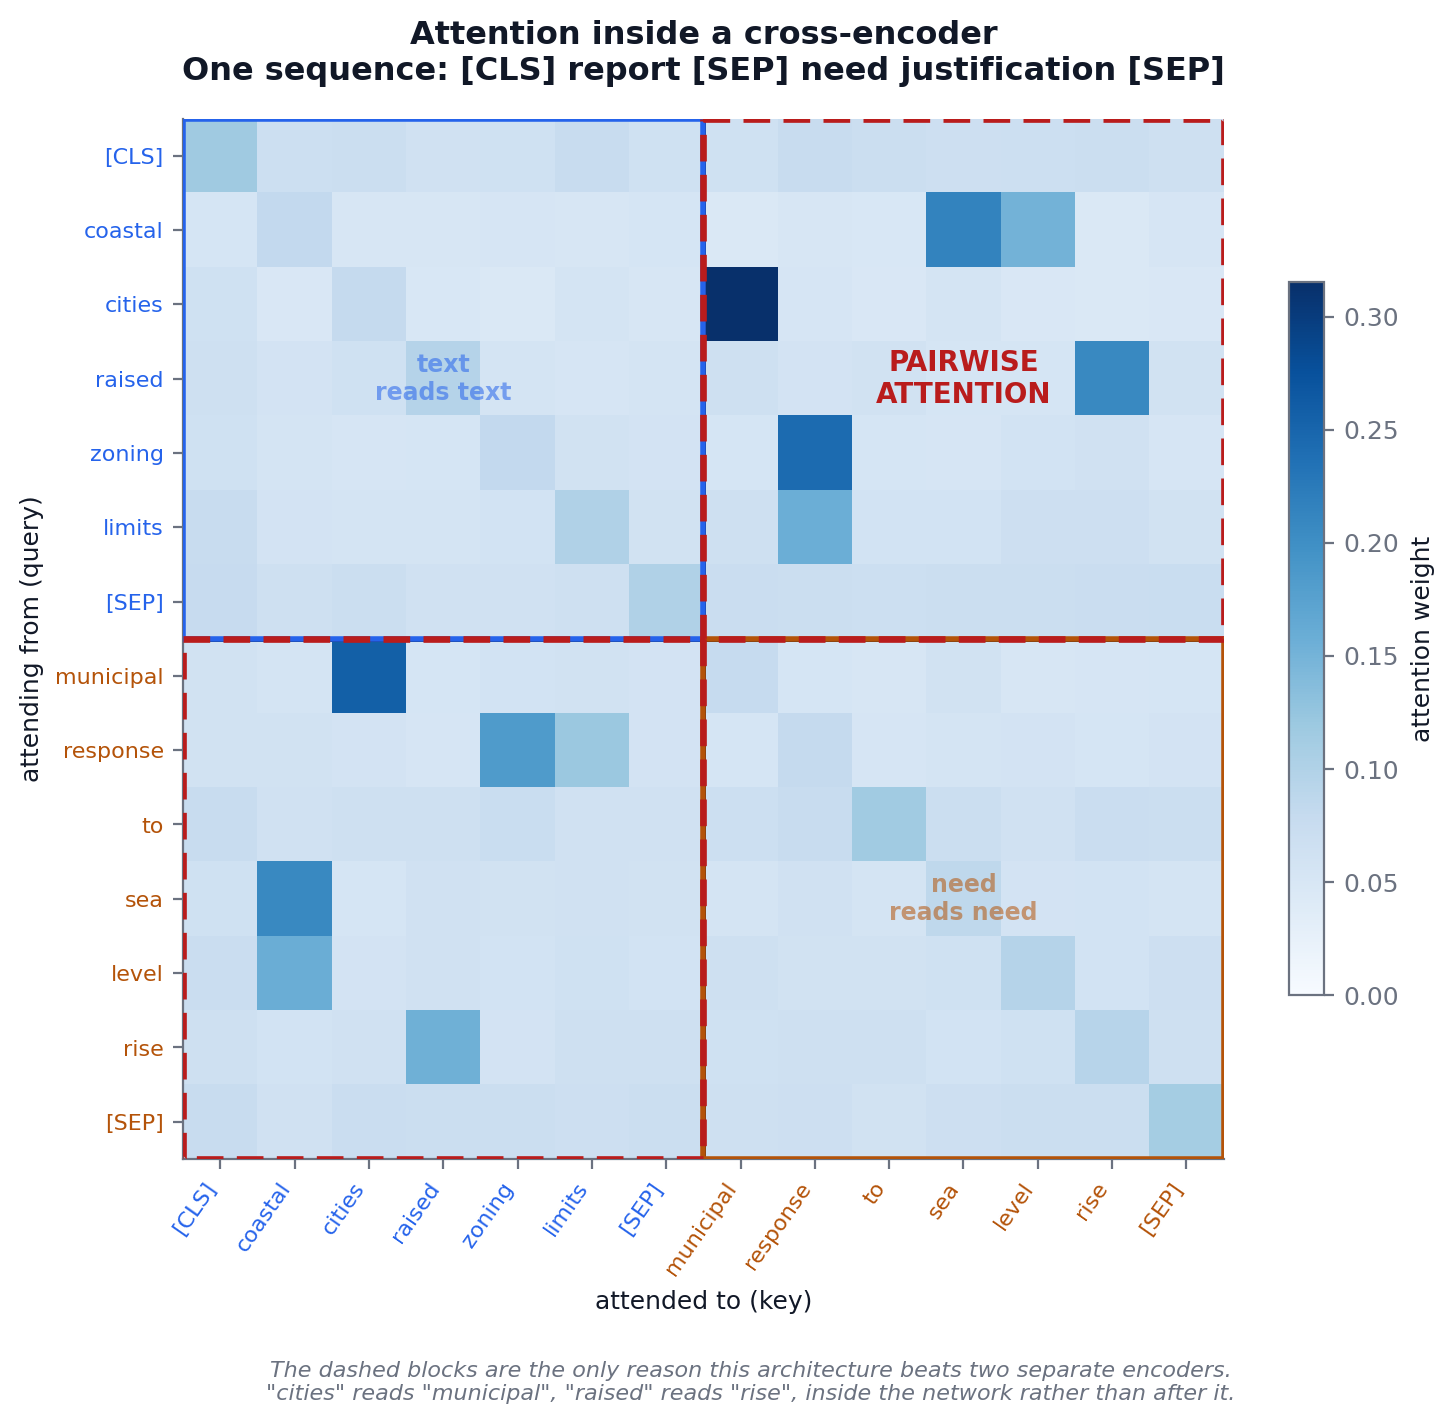
\includegraphics[width=0.86\textwidth]{figures/fig03_cross_segment_attention.png}
\caption{The attention matrix inside a cross-encoder. The two dashed blocks are
the cross-segment regions. This is what ``pairwise attention'' names: tokens in
the text attending directly to tokens in the justification, and back, at every
one of the six layers.}
\label{fig:cross}
\end{figure}

Those dashed blocks are the entire argument for this architecture. The token
``cities'' can attend to ``municipal'' and discover they refer to the same thing.
``raised'' can attend to ``rise'' and register the shared root. None of that is
available to a bi-encoder, which has already compressed each side to a single
768-dimensional vector before any comparison happens. Whatever the two sides
needed to say to each other had to survive that compression.

\subsection{The cost}

The cross-encoder wins on accuracy and loses on cost, for one structural reason.
A bi-encoder can embed all $M$ justifications once, cache them, and reuse the
cache forever. A cross-encoder cannot, because the justification's
representation depends on the text it is paired with. Every pair needs its own
forward pass.

\begin{figure}[H]
\centering
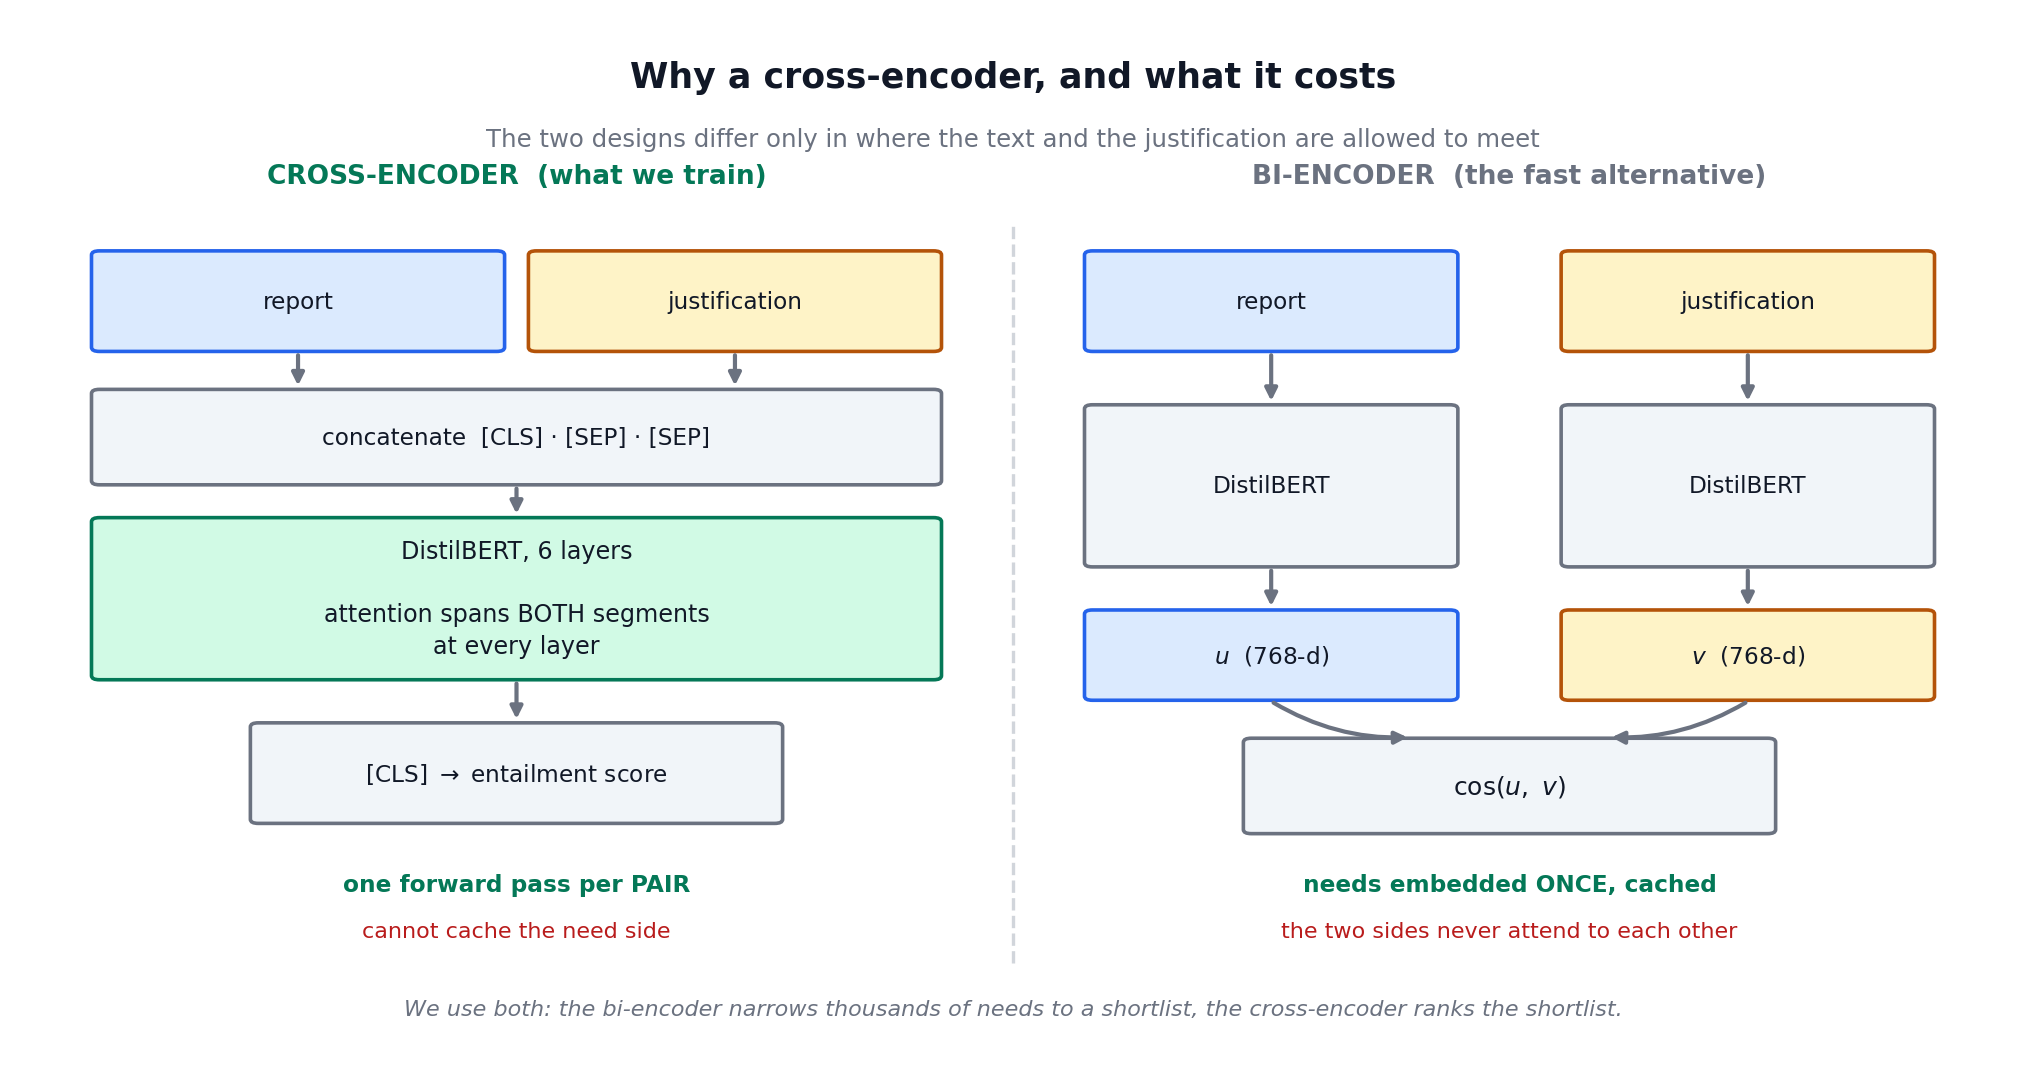
\includegraphics[width=\textwidth]{figures/fig04_encoder_comparison.png}
\caption{The two architectures differ only in where the two inputs are allowed
to meet. That single difference drives both the accuracy gap and the cost gap.}
\label{fig:compare}
\end{figure}

We are not choosing between them. We train the cross-encoder and we use a
bi-encoder to decide which pairs are worth scoring. Section~\ref{sec:serving}
covers the arrangement.

%======================================================================
\section{DistilBERT-MNLI}

The base model is \texttt{DistilBERT-MNLI}. Three pieces of prior work are baked
into that name.

\textbf{BERT} (Bidirectional Encoder Representations from Transformers) is a
transformer trained on raw text by masking random tokens and predicting them.
This gives it general language representations without any task labels.
BERT-base has twelve layers and about 110 million parameters.

\textbf{DistilBERT} is BERT compressed by knowledge distillation, where a
smaller student model is trained to reproduce the larger teacher's outputs. It
keeps six layers and about 66 million parameters, runs roughly 60\% faster, and
retains most of BERT's accuracy. For our purposes the speed matters, because we
will be running many forward passes per document.

\textbf{MNLI} (Multi-Genre Natural Language Inference) is a dataset of 393,000
sentence pairs, each labelled with whether the first sentence entails the
second, contradicts it, or neither. A model fine-tuned on MNLI has already
learned to take two pieces of text and judge their relationship.

\begin{figure}[H]
\centering
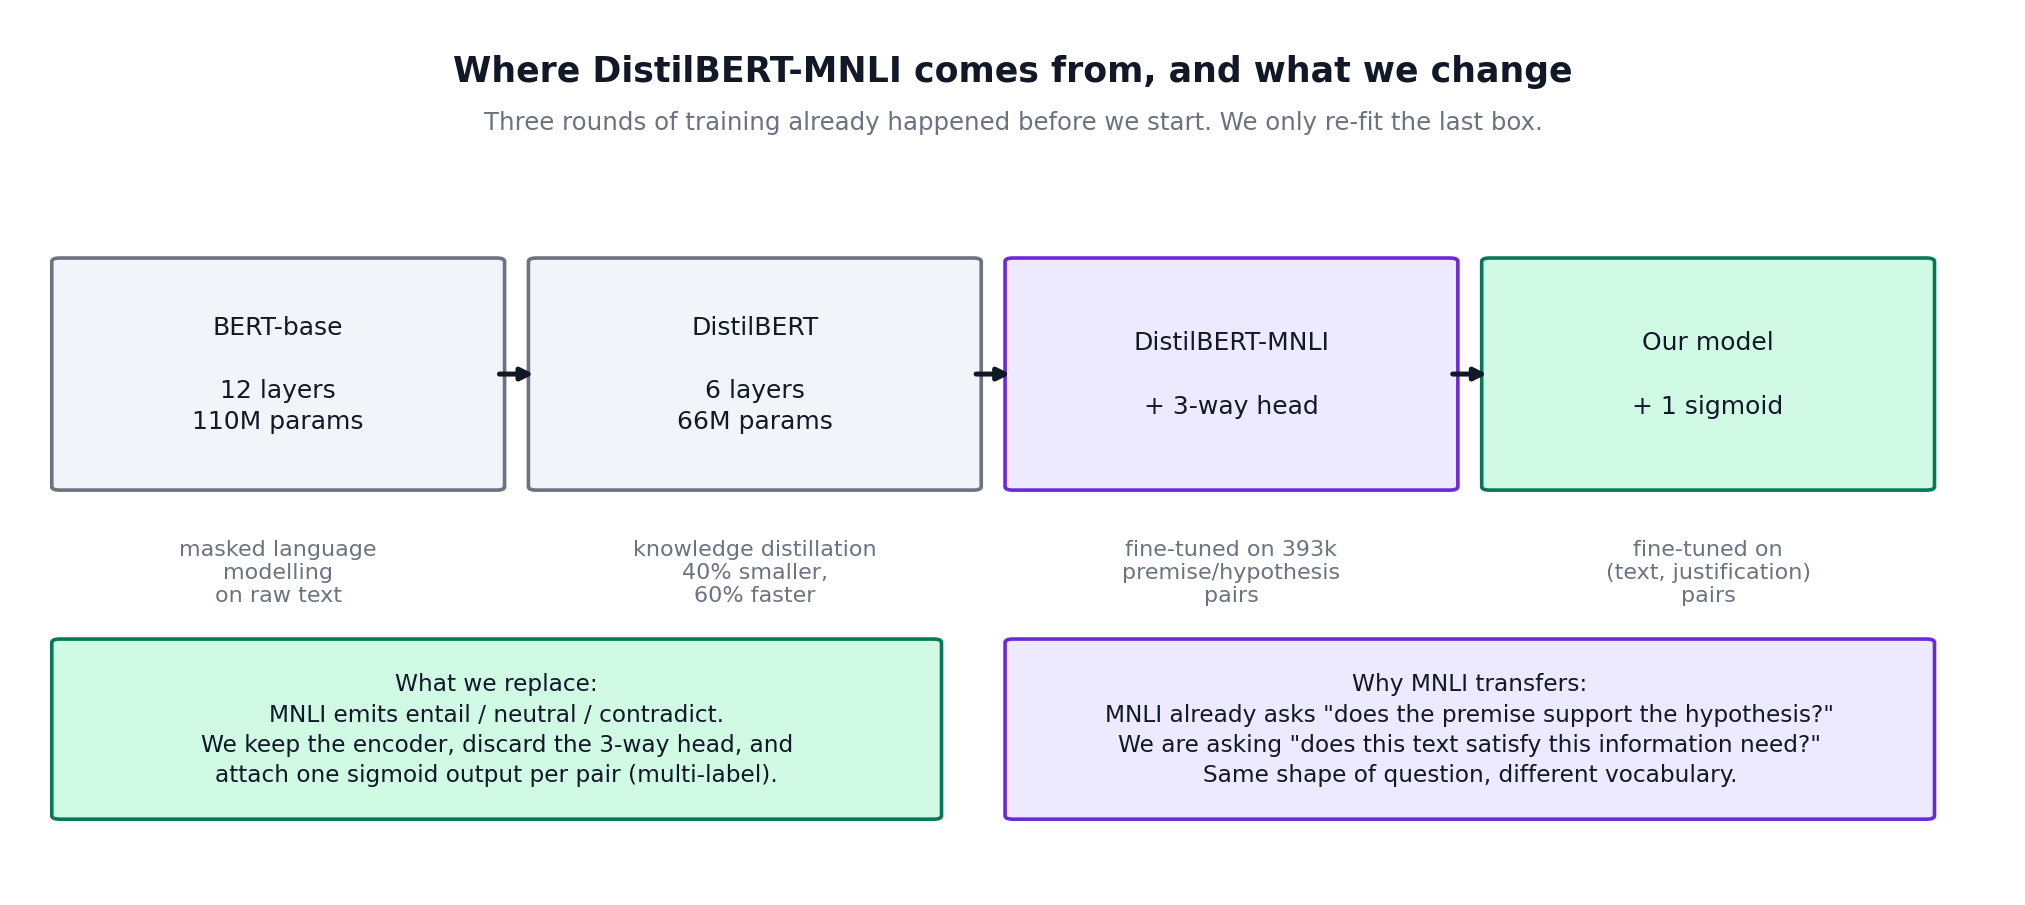
\includegraphics[width=\textwidth]{figures/fig05_distilbert_mnli.png}
\caption{Three rounds of training precede ours. We keep the encoder and replace
only the output head.}
\label{fig:distil}
\end{figure}

Why does MNLI transfer to this task? Because the questions have the same shape.
MNLI asks whether a premise supports a hypothesis. We ask whether a text
satisfies an information need. Both require reading two passages and deciding
whether one licenses the other. The vocabulary differs and the domain differs,
but the reasoning pattern the model has already learned is the one we want.

This is not a small advantage. Starting from MNLI means the model begins with a
usable notion of cross-segment entailment, and fine-tuning only has to adjust it.
In practice it shows up as faster convergence and better performance in the
low-data regime, which is where the rare needs live.

We discard the three-way entailment head and attach a single linear layer with a
sigmoid, producing one probability per pair.

%======================================================================
\section{Training}

\subsection{Input construction}

Each training example is a triple: the text, one justification, and a binary
target. The tokeniser handles the pair encoding directly, inserting the special
tokens and segment identifiers.

\begin{verbatim}
enc = tokenizer(
    text,                       # first segment
    justification,              # second segment
    truncation="only_first",    # cut the text, never the justification
    max_length=256,
    padding="max_length",
    return_tensors="pt",
)
\end{verbatim}

The truncation policy is a real decision. Setting \texttt{only\_first} means we
cut the text when the pair is too long and always keep the justification whole.
That is the right choice here because the justification is short, curated, and
identical across every pair it appears in, whereas the text is long and its
relevant passage may be anywhere. If texts routinely exceed the budget, split
them into overlapping windows and take the maximum score across windows rather
than raising \texttt{max\_length}, since attention cost grows with the square of
sequence length.

\subsection{Loss}

Because each pair is an independent yes-or-no decision, we use binary
cross-entropy on the sigmoid output:

\begin{equation}
L = -\frac{1}{B}\sum_{b=1}^{B}
\Big[ y_b \log p_b + (1 - y_b)\log(1 - p_b) \Big]
\end{equation}

\noindent where $p_b$ is the model's probability for pair $b$ and $y_b \in
\{0,1\}$ is the target. If the sampled ratio still leaves the positives
outnumbered, weight the positive term by the inverse class frequency, or use
focal loss, which down-weights examples the model already gets right.

\subsection{Settings}

\begin{table}[H]
\centering
\small
\begin{tabular}{ll}
\toprule
\textbf{Setting} & \textbf{Value} \\
\midrule
Base checkpoint & \texttt{typeform/distilbert-base-uncased-mnli} \\
Max sequence length & 256 tokens \\
Batch size & 32 pairs \\
Optimiser & AdamW \\
Learning rate & $2\times10^{-5}$ \\
Schedule & linear decay, 10\% warmup \\
Epochs & 3, with early stopping on validation mAP \\
Weight decay & 0.01 \\
Negative sampling & 4 hard, 4 random per positive \\
Mixed precision & fp16 \\
\bottomrule
\end{tabular}
\caption{Starting hyperparameters. The learning rate and the sampling ratio are
the two worth tuning first.}
\end{table}

Three epochs is the usual range for fine-tuning a pretrained encoder. More than
that and the model starts overwriting the pretrained representations it should be
adapting, which shows up as validation performance falling while training loss
keeps dropping.

\begin{figure}[H]
\centering
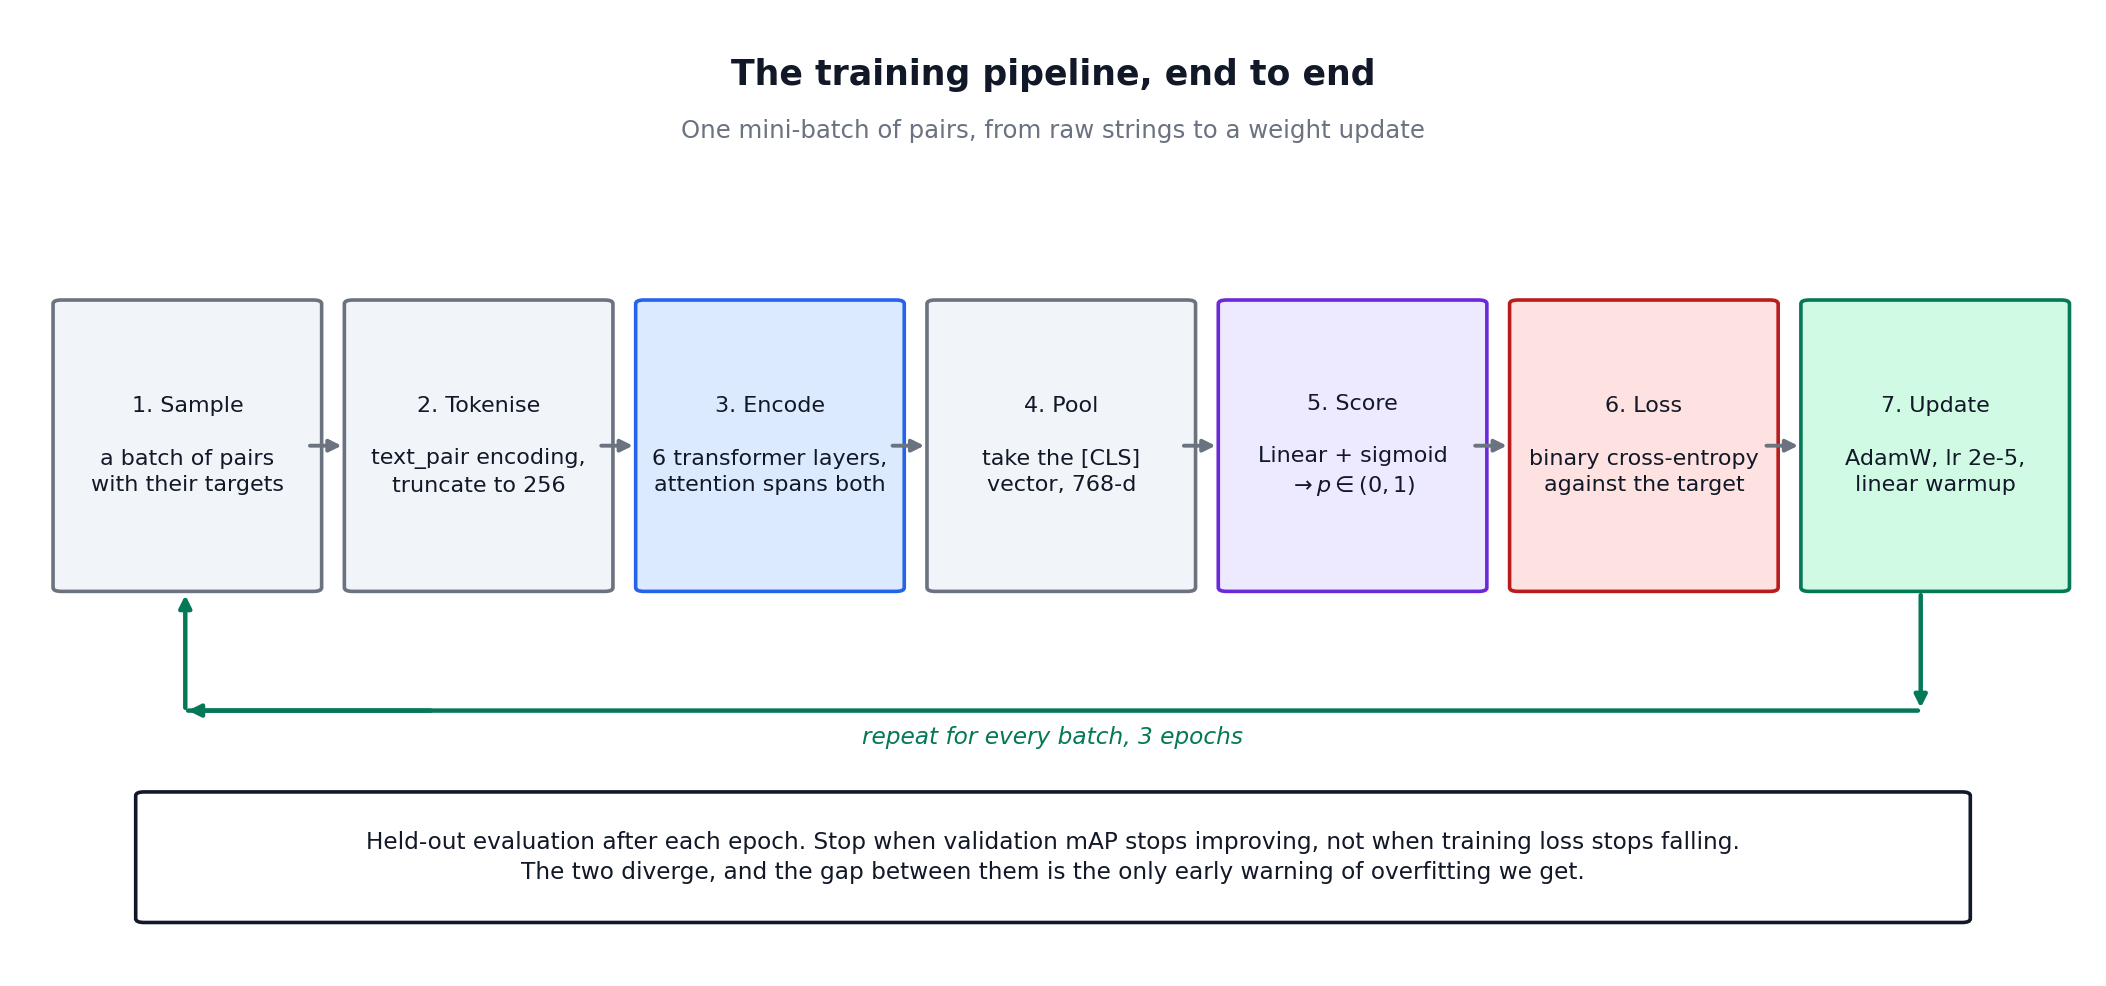
\includegraphics[width=\textwidth]{figures/fig07_training_pipeline.png}
\caption{The full pipeline for one mini-batch.}
\label{fig:pipeline}
\end{figure}

%======================================================================
\section{Evaluation}

Multi-label evaluation is where this kind of project usually goes wrong, because
the convenient metrics hide the interesting failures.

\textbf{Accuracy is not usable.} With thousands of needs and a handful correct,
predicting nothing scores above 99\%.

\textbf{Micro-F1} pools all pair decisions together, then computes precision and
recall. It is dominated by the frequent needs, because they contribute most of
the pairs.

\textbf{Macro-F1} computes F1 per need and averages the results, so a need with
six training examples counts as much as one with nine hundred. The gap between
micro-F1 and macro-F1 is the single most informative number in the evaluation.
A large gap means the model works on common needs and fails on rare ones.

\textbf{Mean average precision} (mAP) evaluates the ranking itself, before any
threshold is applied. That makes it the right metric for model selection, since
it does not depend on a cut point you have not tuned yet.

\textbf{Precision@k and recall@k} answer the operational question directly: if
we show an analyst the top five predicted needs, how often is the right one
there?

\begin{figure}[H]
\centering
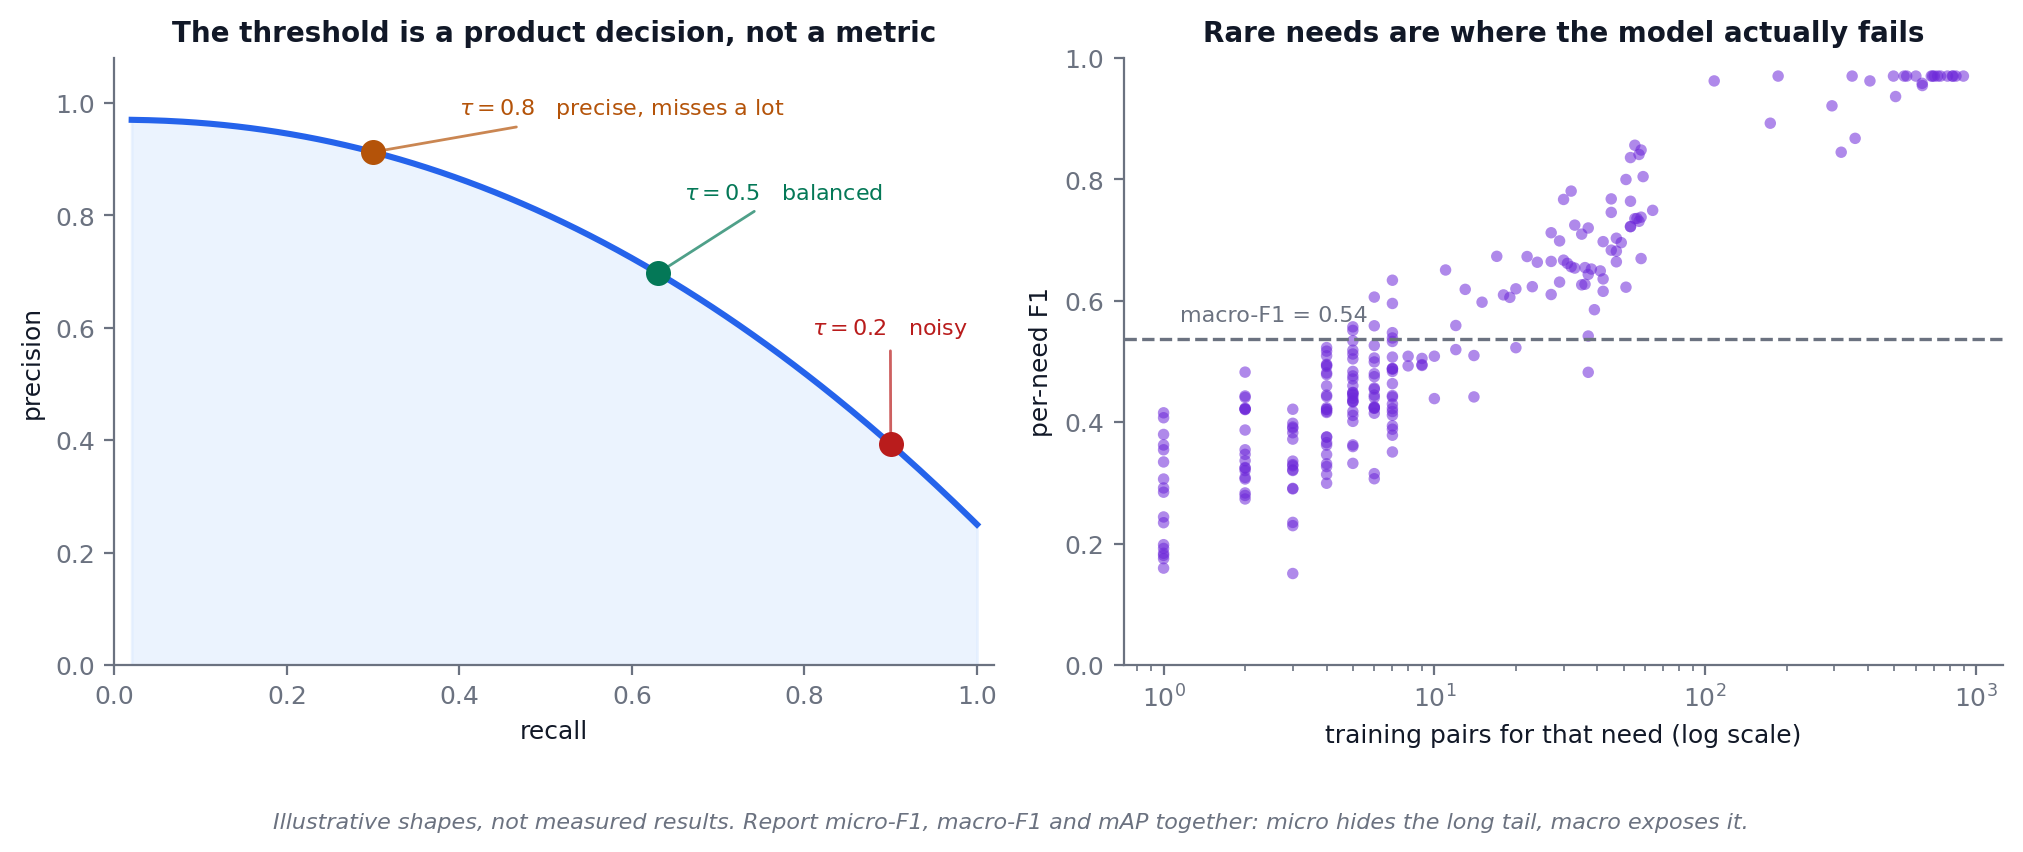
\includegraphics[width=\textwidth]{figures/fig08_multilabel_eval.png}
\caption{Left: the threshold trades precision against recall, and where to sit
on that curve is a decision about how the output gets used, not something the
model determines. Right: performance against training support per need. Both
panels show illustrative shapes rather than measured results.}
\label{fig:eval}
\end{figure}

\subsection{Thresholds}

The model emits a probability. Turning that into a decision requires a threshold
$\tau$, and the right value depends on what happens downstream. If a human
reviews every prediction, favour recall. If predictions are acted on
automatically, favour precision.

Tune $\tau$ on the validation set, never the test set. Consider a separate
threshold per need, since needs differ in base rate and a single global cut point
serves the common ones well and the rare ones badly. Per-need
thresholds need enough validation examples per need to be estimated reliably,
which is itself a reason to check the support distribution before committing.

%======================================================================
\section{Serving at scale}
\label{sec:serving}

With $M > 1{,}000$ needs, scoring every pair means over 1,000 transformer forward
passes per incoming report. At roughly 5 milliseconds each on a GPU that is about
5 seconds per document, so a single pass over the 20,000-report backlog would take
around 28 GPU-hours. Tolerable once as a batch job. Not tolerable interactively,
and not tolerable every time you want to re-score after retraining.

The fix is standard: retrieve, then rerank.

\begin{figure}[H]
\centering
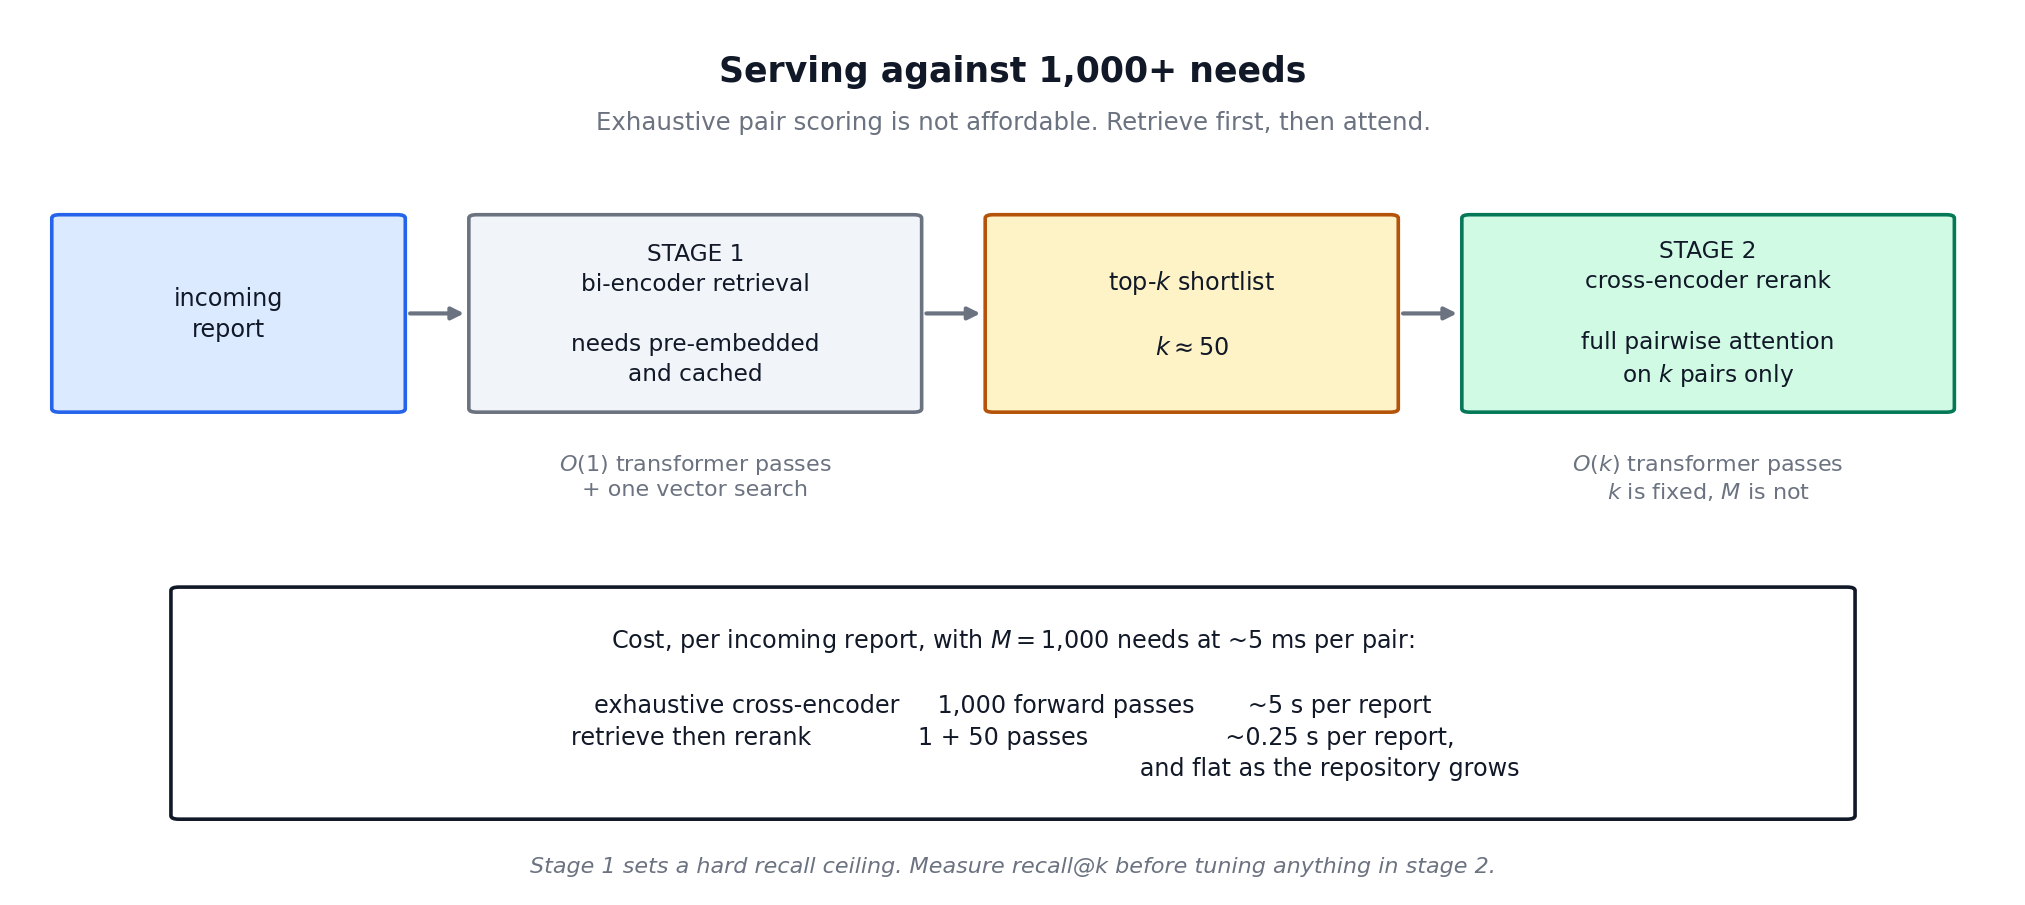
\includegraphics[width=\textwidth]{figures/fig09_serving.png}
\caption{Two-stage inference. Stage one is cheap and approximate, stage two is
expensive and accurate, and the shortlist size $k$ is the dial between them.}
\label{fig:serving}
\end{figure}

Stage one embeds all $M$ justifications once with a bi-encoder and caches them.
An incoming text is embedded once and matched against the cache with approximate
nearest neighbour search, returning the top $k \approx 50$ candidates. Stage two
runs the cross-encoder on those 50 pairs only. Total cost is 51 forward passes
plus a vector search, and it does not grow as the repository grows.

One property of this arrangement deserves stating plainly, because it is easy to
lose track of. \textbf{Stage one sets a hard ceiling on recall.} If the correct
need is not in the top $k$, no amount of cross-encoder quality recovers it.
Measure recall@$k$ for stage one first and report it alongside the end-to-end
number. If recall@50 is 0.88, then 0.88 is the best the full system can do, and
tuning stage two beyond that point is wasted effort.

%======================================================================
\section{Discovering uncited relationships}
\label{sec:discovery}

You said the point is to discover relationships between needs and reports, not
only to reproduce the ones already cited. Section~\ref{sec:labels} showed why
that goal is in tension with the metrics: a real discovery is scored as a false
positive, because the ground truth does not know about it yet.

The resolution is to stop treating the uncited region as noise and start
treating it as a queue.

\begin{figure}[H]
\centering
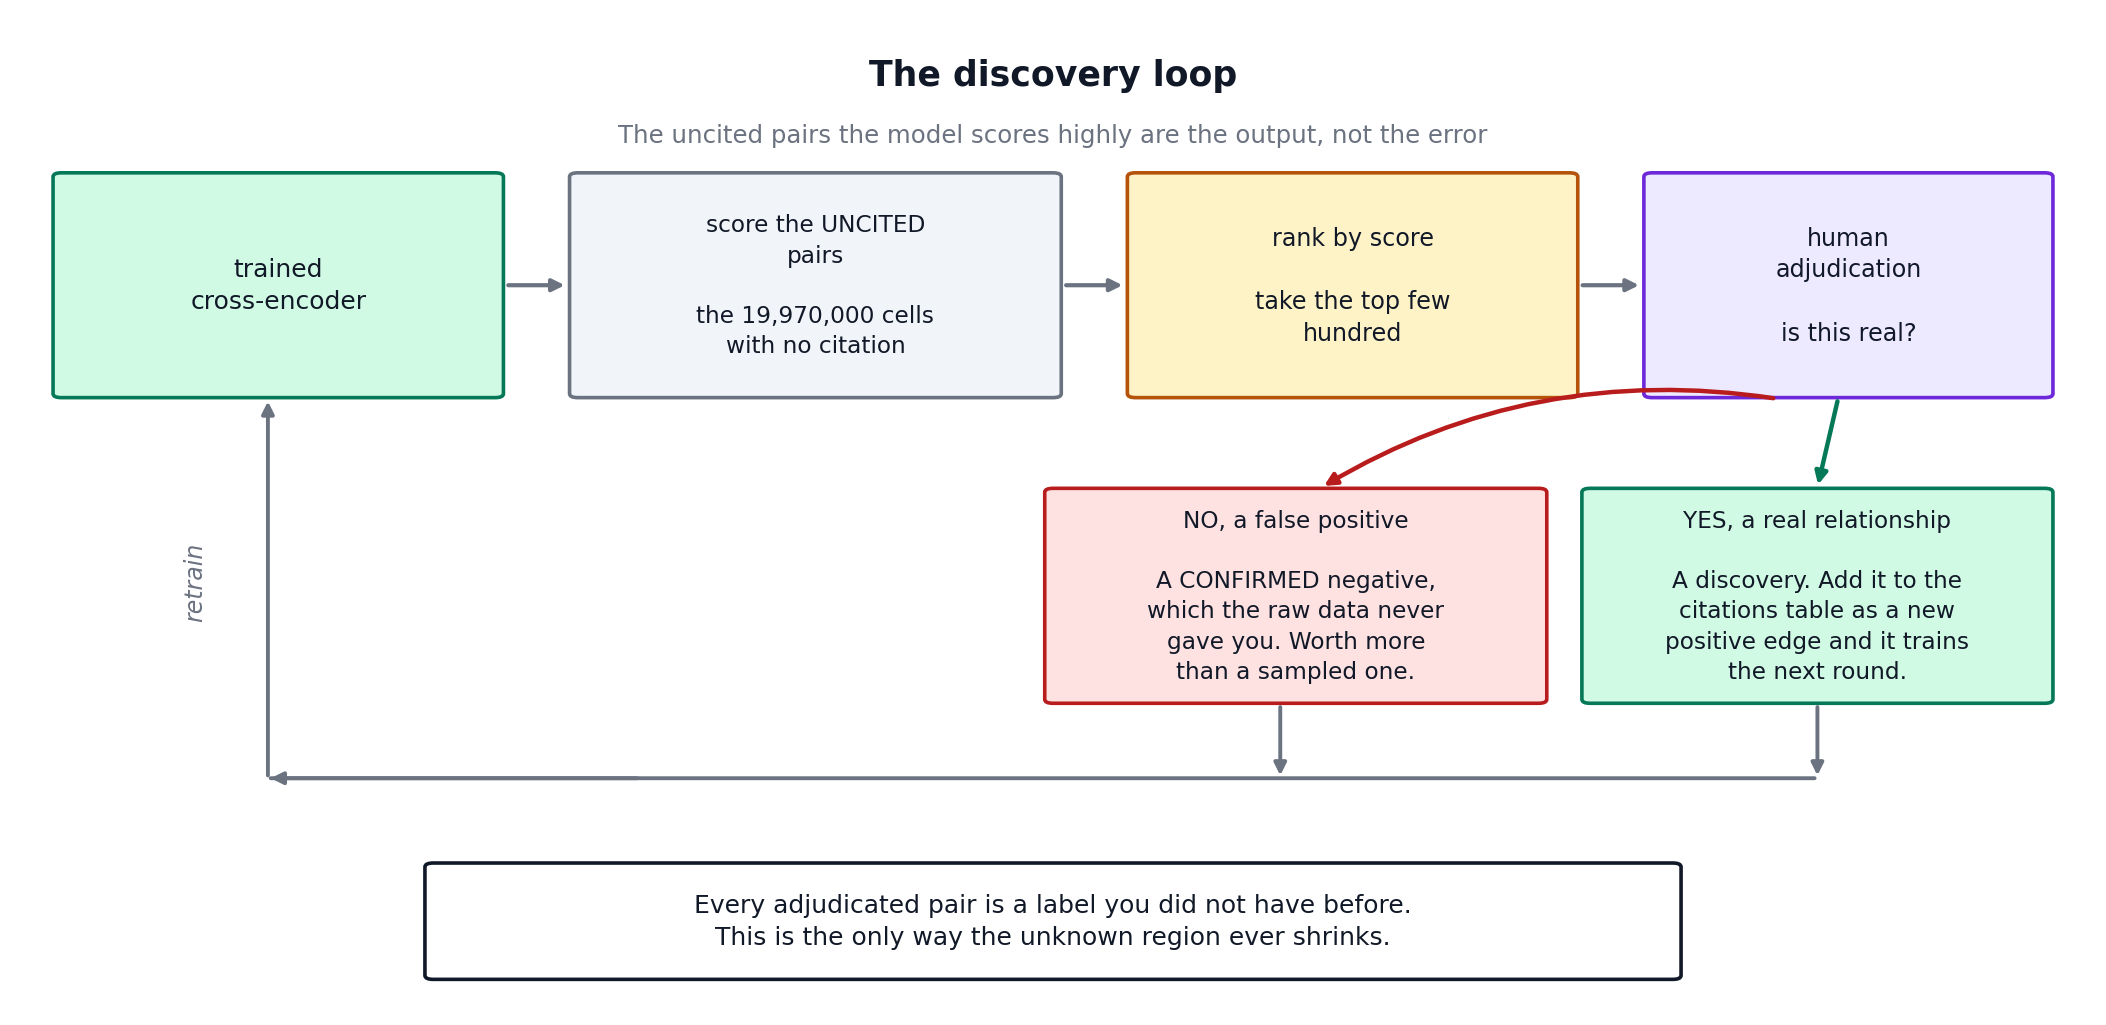
\includegraphics[width=\textwidth]{figures/fig13_discovery_loop.png}
\caption{The discovery loop. Every adjudicated pair is a label that did not
exist before, and adjudication is the only mechanism that shrinks the unknown
region.}
\label{fig:discovery}
\end{figure}

Run the trained model over the roughly 20 million uncited pairs, which the
two-stage design in Section~\ref{sec:serving} makes affordable. Rank them by
score. Take the top few hundred to a human. Each verdict is worth more than a
sampled label:

\begin{itemize}
  \item \textbf{Confirmed relationship.} A discovery, and the deliverable.
        Add it to the citations table as a new positive edge.
  \item \textbf{Confirmed irrelevance.} A true negative, which the raw data
        never contained. These are the highest-value negatives available,
        because they sit exactly where the model is currently wrong.
\end{itemize}

Both outcomes improve the next training round, which is the property that makes
this worth building as a loop instead of a one-shot classifier.

\subsection{Measuring discovery, since standard metrics will not}

Precision and recall against the citation record answer ``does the model
reproduce what authors already wrote down?'' That is worth knowing, and it is not
the question you asked. Three additions.

\textbf{Adjudicated precision at $k$.} Of the top $k$ uncited pairs sent to a
human, what fraction were confirmed real? This is the direct measure of
discovery yield, and it is the number to report to a sponsor. It requires
adjudication effort and no amount of cleverness substitutes for it.

\textbf{Held-out citation recovery.} Hide a random 10\% of known citations,
train without them, then check where they rank among that report's uncited
pairs. If genuine relationships reliably surface in the top 20, the ranking over
the unknown region is trustworthy. This is a proxy for discovery that costs no
human time, and it is the cheapest signal available before any adjudication
happens.

\textbf{Yield curve.} Plot confirmed discoveries against pairs adjudicated. It
will flatten. Where it flattens tells you when to stop reviewing, and that is an
operational answer nothing else gives you.

One caution on the loop. Adding model-proposed edges to the training set makes
the model more confident about the regions it already favours. Keep a fixed
evaluation set of citations that never receives model-proposed edges, so
measurements stay anchored to author judgement rather than to the model's own
prior output.

%======================================================================
\section{What we expect to go wrong}

\textbf{Justification quality is the ceiling.} The model can only match a text
against what the justification says. A need whose justification is one vague
sentence will perform badly no matter how long we train. Before blaming the
model, sort needs by F1 and read the justifications of the worst ones. We expect
this to explain a large share of the errors.

\textbf{Citation is a proxy for relevance, and proxies drift.} An author cites a
report because it was relevant \emph{and} because they found it, could access it,
and remembered it. The model learns all four. If retrieval in your organisation
favours recent or well-indexed reports, the model will inherit that preference
and present it as relevance. Compare per-need precision against report age and
against whatever indexing tier you have. A strong correlation there is a warning.

\textbf{Circularity.} If any justification was written by reading the very
reports now cited against it, the model will do well for a reason that will not
survive contact with new documents. Check when each justification was written
against when its citations were made. \texttt{needs.opened\_on} versus
\texttt{citations.cited\_on} answers this directly. This is the failure mode
most likely to produce a good number and a bad system.

\textbf{Preferential attachment.} Citation records are not uniform. A few needs
attract most citations, and a few reports are cited against many needs. The
model will learn that skew and reproduce it, which makes popular needs look
well-served and rare needs look unserved regardless of the underlying texts. The
micro-to-macro gap detects this. Plot per-need F1 against citation count before
concluding anything about model quality.

\textbf{Distribution shift.} Needs are standing requirements and texts arrive
over time. A model trained on last year's documents may degrade on this year's.
Split by time as well as randomly, and compare, so the size of the shift is known
before deployment.

\textbf{Truncation hiding the evidence.} With \texttt{only\_first} truncation, a
long text whose relevant passage sits past token 200 gets cut before the model
sees it. The failure is silent. Log truncation rates during evaluation.

\textbf{Popularity bias.} If hard negatives are mined with a retriever, frequent
needs get sampled as negatives more often and the model learns to suppress them.
Check whether per-need precision correlates with training frequency, and in
which direction.

%======================================================================
\section{Summary}

The method is one sentence long: score each (report, justification) pair with a
DistilBERT-MNLI cross-encoder, train it with binary cross-entropy on cited
positives and sampled negatives, and serve it behind a bi-encoder that narrows
1,000 candidate needs to fifty.

Everything else in this paper follows from three facts about the problem.

Putting the label on the pair rather than the report lets the justification into
the model, and lets a need opened next month work without retraining. Over 1,000
needs with new ones arriving, that is the difference between a system and a
treadmill.

Concatenating the two sides into one sequence lets attention cross the boundary.
That is what pairwise attention means and why the architecture earns the cost of
scoring pairs instead of caching vectors.

Citations give positives and never negatives. Every negative in training is an
assumption, the assumption is weakest exactly where the model is most useful,
and the pairs that look like errors are the discoveries. Designing around that
is Sections~\ref{sec:labels} and~\ref{sec:discovery}, and it is the part most
likely to be skipped and most expensive to skip.

Three numbers decide whether this works, and the headline F1 is not among them.
The gap between micro-F1 and macro-F1 says whether the long tail of needs is
handled. Recall@$k$ from the retrieval stage is the ceiling on everything
downstream. Adjudicated precision at $k$ is the only direct measure of the
discovery you actually want. Report those three first.

\subsection*{Suggested order of work}

\begin{enumerate}
  \item Build the three tables in Section~\ref{sec:schema}. Count the citations
        and measure the true density before anything else, since every estimate
        in this paper keys off it.
  \item Run the frozen bi-encoder alone and measure recall@50. This costs one
        afternoon, needs no training, and tells you the ceiling. If it is low,
        fix retrieval before touching the cross-encoder.
  \item Train the cross-encoder. It is a few hours on one GPU.
  \item Run the held-out citation recovery test in Section~\ref{sec:discovery}.
        It is the cheapest signal about discovery that needs no human time.
  \item Only then adjudicate a few hundred top-ranked uncited pairs, and
        measure the yield curve.
\end{enumerate}

%======================================================================
\newpage
\section*{Glossary}
\addcontentsline{toc}{section}{Glossary}

\begin{description}[style=nextline,leftmargin=1.2cm]
\item[AdamW] Adam with decoupled weight decay. The optimiser used to update
weights during training.
\item[Attention] The operation that lets each token in a sequence read every
other token, weighted by learned relevance.
\item[BERT] Bidirectional Encoder Representations from Transformers. A
transformer encoder pretrained by predicting masked tokens.
\item[Bi-encoder] An architecture that encodes two inputs separately and
compares the resulting vectors.
\item[BCE] Binary Cross-Entropy. The loss function for independent yes-or-no
predictions.
\item[{[CLS]}] A special token prepended to the input whose final vector is used
as a summary of the whole sequence.
\item[Cross-encoder] An architecture that concatenates two inputs into one
sequence so attention spans both.
\item[DistilBERT] A six-layer compression of BERT produced by knowledge
distillation.
\item[Distillation] Training a small student model to reproduce a larger teacher
model's outputs.
\item[Epoch] One full pass over the training data.
\item[F1] The harmonic mean of precision and recall.
\item[Fine-tuning] Continuing training of a pretrained model on a specific task.
\item[fp16] Half-precision floating point, used to speed up training and reduce
memory.
\item[Gradient descent] The optimisation procedure that repeatedly steps
parameters in the direction that lowers the loss.
\item[Hard negative] A negative example that a retrieval model ranks highly,
making it informative for training.
\item[Learning rate] The size of each gradient descent step.
\item[Macro-F1] F1 computed per class and averaged, giving rare classes equal
weight.
\item[mAP] Mean Average Precision. A ranking metric that does not depend on a
decision threshold.
\item[Micro-F1] F1 computed over all decisions pooled together, dominated by
frequent classes.
\item[MNLI] Multi-Genre Natural Language Inference. A 393,000-pair dataset for
judging entailment between two sentences.
\item[Multi-label] A setting where each input may carry several labels at once,
as opposed to exactly one.
\item[NLI] Natural Language Inference. The task of deciding whether one passage
entails, contradicts, or is neutral toward another.
\item[Overfitting] Fitting the training data in ways that do not generalise.
\item[Positive-unlabeled learning] A setting with confirmed positive labels and
no confirmed negatives, where unlabeled examples are a mixture of true negatives
and undiscovered positives.
\item[Preferential attachment] The tendency of already-popular items to attract
further links, which makes citation records skewed rather than uniform.
\item[Query, key, value] The three projections of each token that attention uses
to compute its weights and outputs.
\item[Recall@k] The fraction of correct answers appearing in the top $k$
retrieved candidates.
\item[{[SEP]}] A special token marking the boundary between the two segments of a
pair.
\item[Sigmoid] A function mapping any real number to the range $(0,1)$, used for
independent probability outputs.
\item[Softmax] A function turning a vector of scores into probabilities that sum
to one.
\item[Token] The unit of text the model operates on, typically a word or
sub-word piece.
\item[WordPiece] The sub-word tokenisation scheme used by BERT and DistilBERT.
\end{description}

\end{document}
